\documentclass[12pt]{Definitions/academia}

\usepackage{hyperref}
\usepackage{color}
\usepackage{refstyle}
\usepackage{float}
\usepackage{url}
\usepackage{varwidth}
\usepackage{amsmath}
\usepackage{graphicx}
\usepackage{geometry}
\usepackage{algorithm}
\usepackage{algpseudocode}
\usepackage{setspace}
\onehalfspacing
\usepackage{textcomp}
\setlength{\abovecaptionskip}{3pt}
\setlength{\belowcaptionskip}{3pt}




\begin{document}

%%%%%%%Author Note%%%%%%%%%%%%%%%%%%%%%%%%%%%%%%%%%%%%%%%%%%%%%%%%%%%%%%%%%%%%%%%%%%%%%%%%%%%%%%%%%%%

%Academia.edu Publishing LaTeX Template -- Please follow this optional template to format your article. You can also refer to article formatting instructions in the author guidelines
%For all sections, check the author guidelines to see if a specific section is required for your article type.

\articletype{Research article}
\proofstage{Template or Preprint}
\jName{Journal Name}

%%%%%%%%%%%%%%%%%%%%%%%%%%%%%%%%%%%%%%%%%%%%%%%%%%%%%%%%%%%%%%%%%%%%%%%%%%%%%%%%%%%%%%%%%%%%%%%%%%%%%%


\title{Predicting the Temperature Class for Climate Change in Different Zones
Using Grammatical Evolution}

%No Longer than 96 Characters (Inclusive of Spaces)

\author{$^{1}$Constantina Kopitsa, $^{1*}$Ioannis G. Tsoulos, $^{1}$Vasileios Charilogis}

\maketitle

\affiliation{$^{1}$Department of Informatics and Telecommunications,
University of Ioannina, Greece. }

\noindent $^{*}$Correspondence:  Ioannis G. Tsoulos
\email{$^{*}$itsoulos@uoi.gr}

\section*{Abstract}
Climate change is no longer a distant or hypothetical concern, but
it has become an immediate reality with tangible consequences and
impacts on  the planet and on all living organisms within its ecosystems.
Since 1969, the global surface temperature has been breaking previous
records almost annually, with NASA\textquoteright s final measurement
for 2024, indicating an increase of approximately 2.65  degrees Fahrenheit
or 1.47 Celsius, in global temperature. These findings indicate that
we have reached the critical thresholds established by the United
Nations, the scientific community, and member states through the Paris
Agreement of 2015. On this occasion, in this study, we aim to develop
a comprehensive understanding of climate change, and more specifically
of its environmental impacts across seven regions located in different
climatic zones. Significant emphasis is placed on highlighting the
rate at which climate change has altered annual temperature patterns
during the period 1995--2025 across the Congo region, Saudi Arabia, Greece,
Turkey, Reykjavik in Iceland, the Arctic Archipelago of Svalbard,
and Cape Town in South Africa. To achieve this, we evaluated multiple
modeling techniques and proposed the use of Grammatical Evolution
with rule-based construction as the most suitable approach. GENCLASS,
demonstrates robust and systematic superiority over the considered
baselines (MLP, RBF, SVM, and NNC) across all datasets, achieving
the lowest average classification error and indicating strong cross-regional
generalization. Our experiments yielded highly robust results, with
an average error rate of 1.66\% and a classification accuracy of 98.34\%
for predicting climate change categories. These outcomes were further
confirmed through established validation techniques, reinforcing the
reliability of the model\textquoteright s performance.

\keywords{Genetic Algorithms; Grammatical Evolution; Machine Learning;
Climate Change.}

\section{Introduction}\label{sec1}

The power of nature and its capacity to respond when ecological balances
are disrupted has long been recognized. A striking early example appears
in  Persians by Aeschylus, a classical tragedy written in 472 BCE
that recounts the historical events of 480 BCE \textit{\cite{Aeschylus,Aeschylus-1}}.
The play depicts the environmental and human catastrophes that afflicted
the Persian army during its chaotic retreat, following acts that violated
the natural world. Historical sources describe these transgressions,
including the \textquotedblleft chaining\textquotedblright{} of the
Bosporus through the construction of a floating bridge, the plundering
of agricultural lands to sustain their vast forces, and the burning
and devastation of forests and plains---actions intended to deprive
local populations of essential resources.\\
 Such accounts illustrate
that every action elicits a reaction, even from nature itself, which
does not remain a passive observer but acts as a regulating force
that safeguards the planet\textquoteright s equilibrium.

Recent scientific consensus confirms that anthropogenic factors, especially
fossil fuel combustion, deforestation, and industrial emissions,play
a pivotal role in driving climate change and its associated extreme
events. \\
In summary, climate change has been linked to extreme natural
disaster events, including heat waves and cold spells, droughts, tropical
storms and high winds, river floods, coastal floods \textit{\cite{Dey 2021}}
and wildfires \textit{\cite{Kopitsa,United Nations  2022}}. In particular,
according to the United Nations, climate change refers to long-term
alterations in temperature and weather patterns. While such variations
may occur naturally---stemming from fluctuations in solar activity
or major volcanic eruptions---human activities have emerged as the
predominant cause since the 19th century. \\This anthropogenic influence
is primarily attributed to the extensive combustion of fossil fuels,
including coal, oil, and natural gas \textit{\cite{United Nations}}.
As will be demonstrated through the data presented below, climate
change has entered an irreversible trajectory, with each passing year
bearing witness to phenomena that repeatedly set new temperature records.
Nevertheless, notable efforts have been made in the past---through
treaties, regulations, targets, and constraints---aiming to reduce
carbon dioxide emissions in an attempt to intercept climate change
at a critical threshold.\\
 Specifically, the 1992 UN Conference of Environment
and Development set as its ultimate objective \textquotedblleft the
stabilization of greenhouse gas concentrations in the atmosphere\textquotedblright{}
\textit{\cite{United Nations 1992}}. In 1997, the Kyoto Protocol
was adopted with the aim of committing industrialized nations and
economies in transition to limit and reduce greenhouse gas (GHG) emissions,
based on individually agreed targets. The overarching Convention,
however, merely requires these countries to implement mitigation policies
and measures, and to submit periodic reports \textit{\cite{United Nations 1997}.}\\
In 2015, the Paris Agreement articulated long-term goals intended
to guide 195 Parties in substantially reducing global greenhouse gas
emissions. Its central aim is to constrain the rise in global temperatures
to well below 2\textdegree C above pre-industrial levels, while encouraging efforts
to limit the increase to 1.5\textdegree C. Achieving these targets is recognized
as a critical step towards significantly mitigating the risks and
adverse impacts associated with climate change \textit{\cite{United Nations 2015}.}\\
Although we briefly observed the emergence of more environmentally
conscious actions in the past, in the year 2025, NASA's data
indicate that the debate has shifted to whether humanity will surpass
the critical threshold of 1.5\textdegree C or 2.7\textdegree F global temperature \textit{\cite{NASA 2024}}.

In the field of climate change projections, numerous studies have
been conducted. The first scientifically documented prediction of
climate change was made in 1896, by Svante Arrhenius, in his work
\textquotedblleft On the Influence of Carbon Acid in the Air upon
the Temperature of the Ground\textquotedblright{} \textit{\cite{Arrhenius}}.
The aforementioned scholar estimated that the combustion of fossil
fuels could ultimately emit sufficient carbon dioxide to raise the
Earth\textquoteright s temperature by approximately 5 - 6 degrees. Since then, approximately 130 years have passed; nevertheless,
the fundamental physics underlying these calculations has remained
unchanged. What has evolved are the techniques employed in our projections,
which have become considerably more detailed and precise \textit{\cite{Rolnick 2022}}.
It is evident that climate change is intrinsically linked to global
warming and the increasing occurrence of natural disasters, such as
wildfires, floods, droughts, extreme weather events, landslides, and
storms.

In this context, we will refer to several studies on climate change
and forest fires, such as: Koulelis et al., in 2023, conducted a study
reviewing the impacts of climate change on Greek forests, examining
factors such as climate trends, forest management practices, biodiversity,
genetics, insect activity, and wildfires, drawing upon data from the
Scopus and Mendeley databases as well as official reports \textit{\cite{Koulelis 2023}}.
The findings of Rovithakis et al., in 2022, indicate that fire danger
is projected to progressively intensify in the future, particularly
under the high-end climate change scenario \textit{\cite{Rovithakis 2022}}.
Xepapadeas et al., in 2024, investigated the climatic factors shaping
forest fire occurrence and projected future changes in the frequency
of such events \textit{\cite{Xepapadeas 2024}}.

Comparable studies have linked floods to climate change, such as:
Knox, in 2000, reported that flood chronologies from multiple regions
indicate that periods of rapid climate change tend to coincide with
more frequent occurrences of large and extreme flooding events \textit{\cite{Knox 2000}}.
Milly et al., in 2002, found that the frequency of major floods increased
significantly throughout the twentieth century \textit{\cite{Milly 2002}}.
Angra et al., in 2022, demonstrated that climate change manifests
differently even in adjacent areas, with direct implications for forest
fire and flood risk \textit{\cite{Angra 2022}. }

Subsequently, we will discuss studies addressing drought and its linkage
to climate change, including: Cook et al., in 2018, projected that
rising temperatures will heighten both the risk and severity of drought
across large parts of the subtropics and mid-latitudes in both hemispheres,
as a result of regional declines in precipitation combined with widespread
warming \textit{\cite{Cook 2018}}. Stathi et al., in 2023, reported
that the marked increase in temperature could lead to drought episodes
\textit{\cite{Stathi 2023}}. Yuan et al., in 2023, observed that
flash droughts---developing unusually rapidly in contrast to the
more gradual archetypal droughts, are increasingly becoming the new
normal \textit{\cite{Yuan 2023}.}

Consequently, research on rising temperatures has attracted significant
scientific interest. Subsequently, we will present studies that focus
on the field of climate change, specifically on the projection of
such meteorological phenomena.\\
 Kretschmer et al., published in 2017,
a novel empirical method for predicting Extreme Stratospheric Polar
Vortex States by combining a response guided community detection approach
with a causal discovery algorithm \textit{\cite{Kretschmer 2017}}.
Kambezidis et al., in 2021, analyzed future thermal sensation in Greece
\textit{\cite{Kambezidis 2021}.} Lindsay et al., in 2025, highlighted
the world's rising temperature\textit{\cite{Lindsey 2025}}. Mansfield
et al., in 2020, introduced a machine learning approach that leverages
a unique dataset of existing climate model simulations to identify
relationships between short-term and long-term temperature responses
under different climate forcing scenarios \textit{\cite{Mansfield 2020}}.
Haggag et al., in 2021, demonstrated the application of the developed
model by linking flood disaster data from the Canadian Disaster Database
with climate change indices for Ontario, which were then used to train,
test, and validate the model\textit{\cite{Haggag 2021}}. Haq, in
2022, developed and optimized the Climate Deep Long Short-Term Memory
(CDLSTM) model to forecast temperature and rainfall values across
all Himalayan states\textit{\cite{Haq 2022}}. Slater et al., in 2023,
reviewed recent advances in hybrid hydroclimatic forecasting and delineated
key challenges and opportunities for future research \textit{\cite{Slater 2023}.}
Singh Bist et al., in 2024, research introduced an innovative method
for predicting climate change by employing deep learning techniques\textit{\cite{Bist 2024}}.
Gautam et al., in 2025, advanced the examination of climate time series
data and enhance its analysis through deep learning methods\textit{\cite{GAUTAM 2025}. }

A method that constructs classification rules using the technique
of Grammatical Evolution \textit{\cite{O'Neill 2002}} is proposed
here for predicting climate change categories. The Grammatical Evolution
procedure can be considered as a genetic algorithm\textit{\cite{Kramer 2017}},
where the chromosomes are series of integer values the representing
the production rules of the provided Backus-Naur form (BNF) grammar\textit{\cite{Backus 1959}}.
The Grammatical Evolution procedure has been used successfully in
a series of practical problems, such as data fitting problems \textit{\cite{Ryan 1998,Neill 1999}},
issues appeared in economic problems \textit{\cite{Brabazon 2006}},
issues regarding network security \textit{\cite{Sen 2009},} problems
regarding the quality of water\textit{\cite{Chen 2008}}, medicine
problems\textit{\cite{Hidalgo 2014}}, evolutionary computation \textit{\cite{Tavares 2012},}
problems that appear in data centers\textit{\cite{Zapater 2016}},
solution of trigonometric problems\textit{\cite{Ryan 1998-1}}, automatic
composition of music \textit{\cite{de la Puente 2002}}, construction
of the architecture of neural networks \textit{\cite{De Campos 2016,Soltanian 2022},}
production of numerical constants \textit{\cite{Dempsey 2007},} playing
video games\textit{\cite{Galv=0000E1n-L=0000F3pez 2010,Shaker 2012}},
energy problems\textit{\cite{Mart=0000EDnez=002010Rodr=0000EDguez 2020}},
combinatorial optimization\textit{\cite{Sabar 2013},} cryptography
problems\textit{\cite{Ryan 2022},} construction of decision trees\textit{\cite{Pereira 2021},}
electronic problems\textit{\cite{Castej=0000F3n 2018} }etc.


{The motivation for this research stems from the well- established fact that climate change affects the sustainability of our planet through its harmful impacts and the intensification of natural-disaster phenomena, as discussed in the studies referenced above. Beyond this, our objective was twofold: first, to examine the progression of climate change through direct statistical analysis, and second, to assess the current stage relative to internationally established climate targets and present our findings accordingly.
The most effective and comprehensible way to achieve this was to begin with a separate statistical analysis for each region of interest, which formed the basis for defining the two temperature-increase classes. The definition of these two classes serves a dual purpose: on the one hand, it balances the dataset, and on the other, it aligns with the climate thresholds set by international environmental institutions.}

This paper proposes the application of a technique for automatically
generating classification rules to predict climate change classes
in various regions of our planet. These rules are expressed in a C
- like programming language and they can also detect hidden correlations
between the features of the problem and use only those features that
contain the most important information for the correct classification
or patterns of the objective problem. \\
In contrast to conventional
AI methods, the proposed framework produces interpretable C\nobreakdash-like
rules while simultaneously performing implicit feature selection,
enabling more explainable and efficient climate\nobreakdash-prediction
models.\\
The rest of this manuscript is organized as follows: the used dataset
and the incorporated methods used in the conducted experiments are
outlined in section \ref{sec:Materials-and-methods}, the experimental
results are shown and discussed in section \ref{sec:Results} and finally a
detailed discussion is provided in section \ref{sec:Conclusions}.

\section{Materials and Methods\label{sec:Materials-and-methods}}

In this section, a detailed presentation of the datasets used as well
as the machine learning techniques used in the experiments performed
will be provided.

\subsection{\textmd{Impacts of Climate Change in Natural Disasters}}
In order to present the impacts of climate change on natural disasters,
visual representations of the planet\textquoteright s average temperature
are provided for the years 1881, 1995, and 2024. Visualization is
from NASA Goddard's Scientific Visualization Studio \cite{NASA 2024}. 
as seen in Figures
\ref{fig:NASA-Global-Temperature-1881}, \ref{fig:NASA-Global-Temperature-1881}, \ref{fig:NASA-Global-Temperature-2024}.\\
{At this point, it should be noted that the purpose of this figures is primarily illustrative and informational with respect to climate change, specifically the global increase in temperature. The figures depicts the rapid rise in Earth's temperature following the Industrial Revolution, in order to make it clear that the planet has been gradually warming over time.}\clearpage


\textquotedblleft This color-coded map shows changing global surface
temperature anomalies. Normal temperatures are shown in white, higher
than normal temperatures in red and lower than normal temperatures
in blue\textquotedblright .\\

\begin{figure}
	\centering
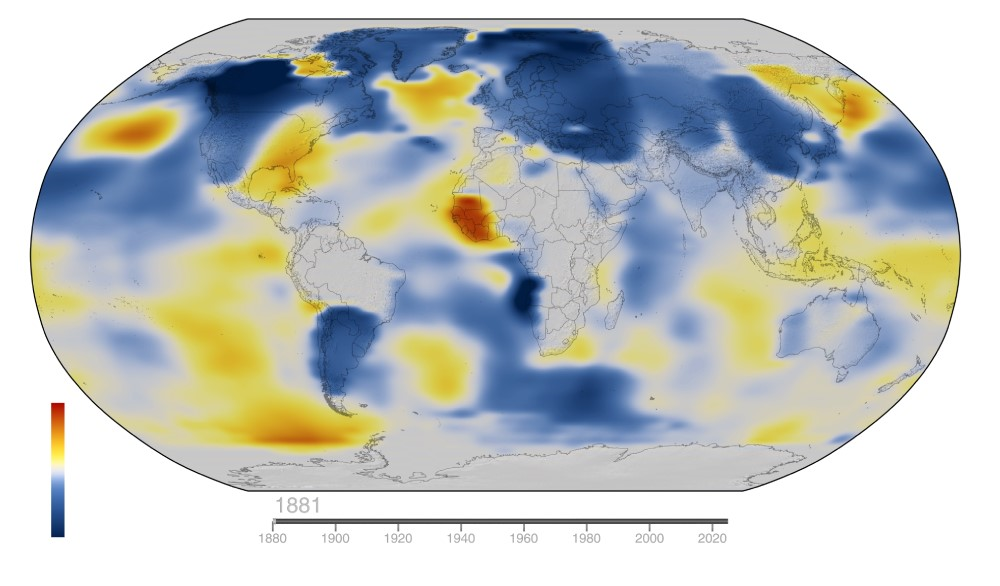
\includegraphics{1881-300dpi}
\caption{Global Temperature 1881, source by NASA Earth Indicator. Available from https://science.nasa.gov/earth/explore/earth-indicators/
	global-temperature/ 
	   \label{fig:NASA-Global-Temperature-1881}}


\vspace{7pt} 

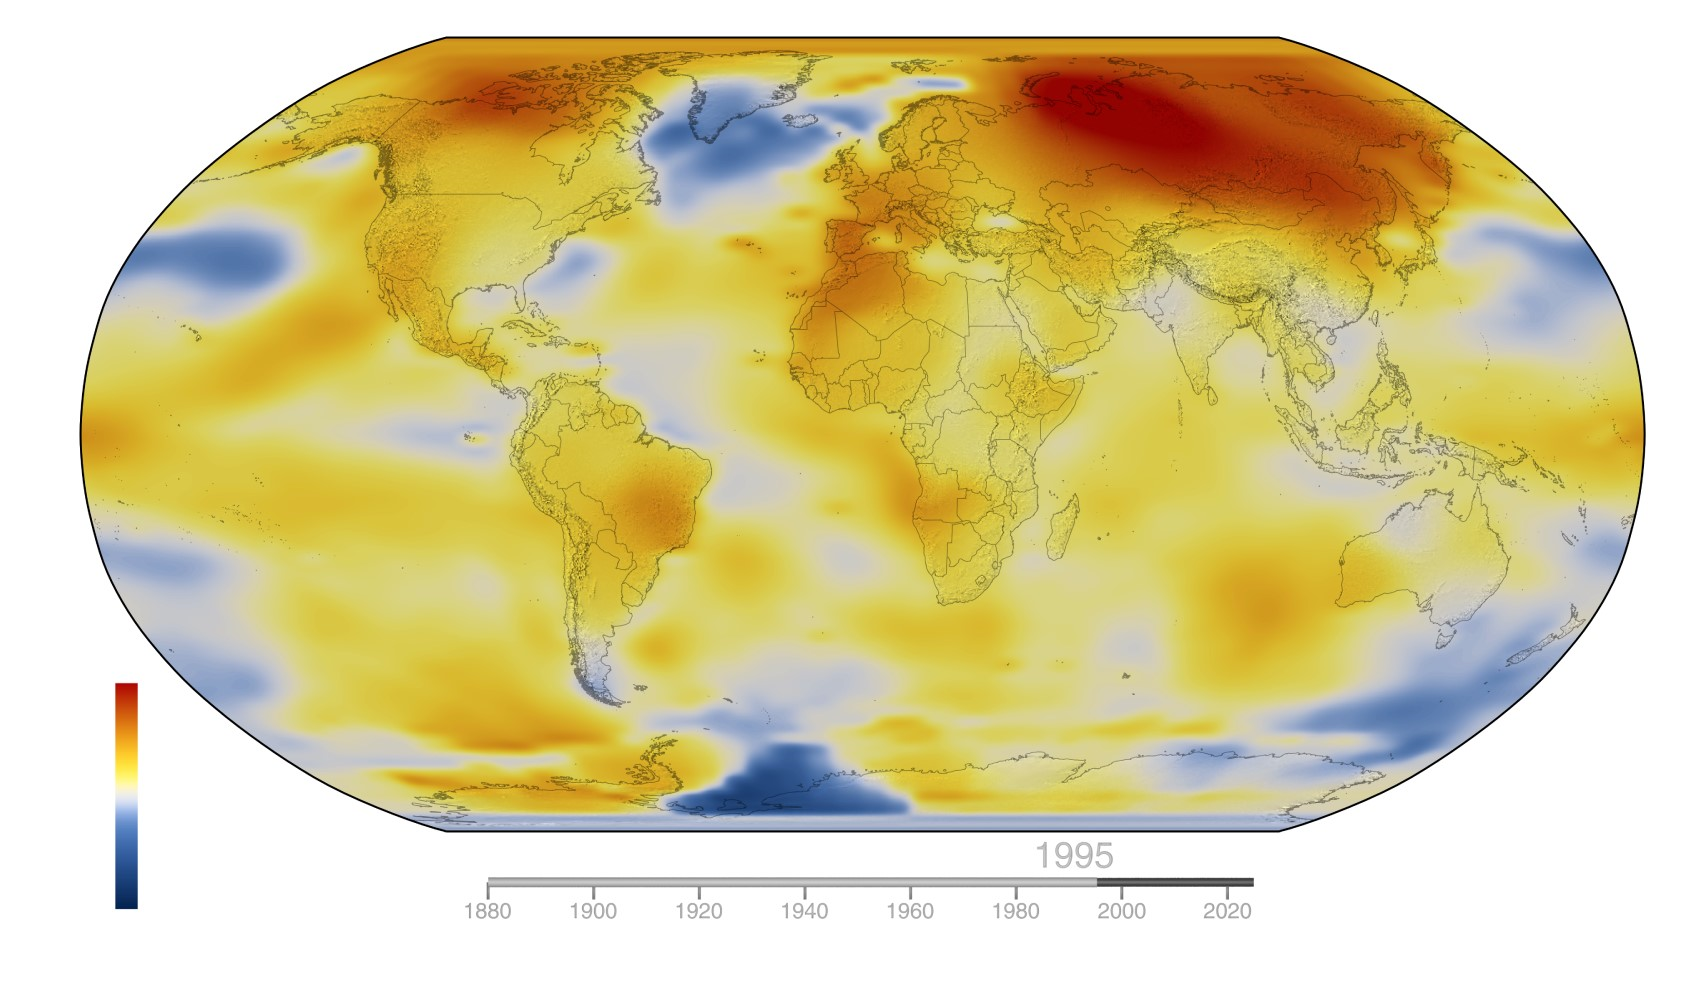
\includegraphics{1995-300dpi}\caption{Global Temperature 1995, source by NASA Earth Indicator. Available from https://science.nasa.gov/earth/explore/earth-indicators/
	global-temperature/\label{fig:NASA-Global-Temperature-1995}}

\vspace{7pt}

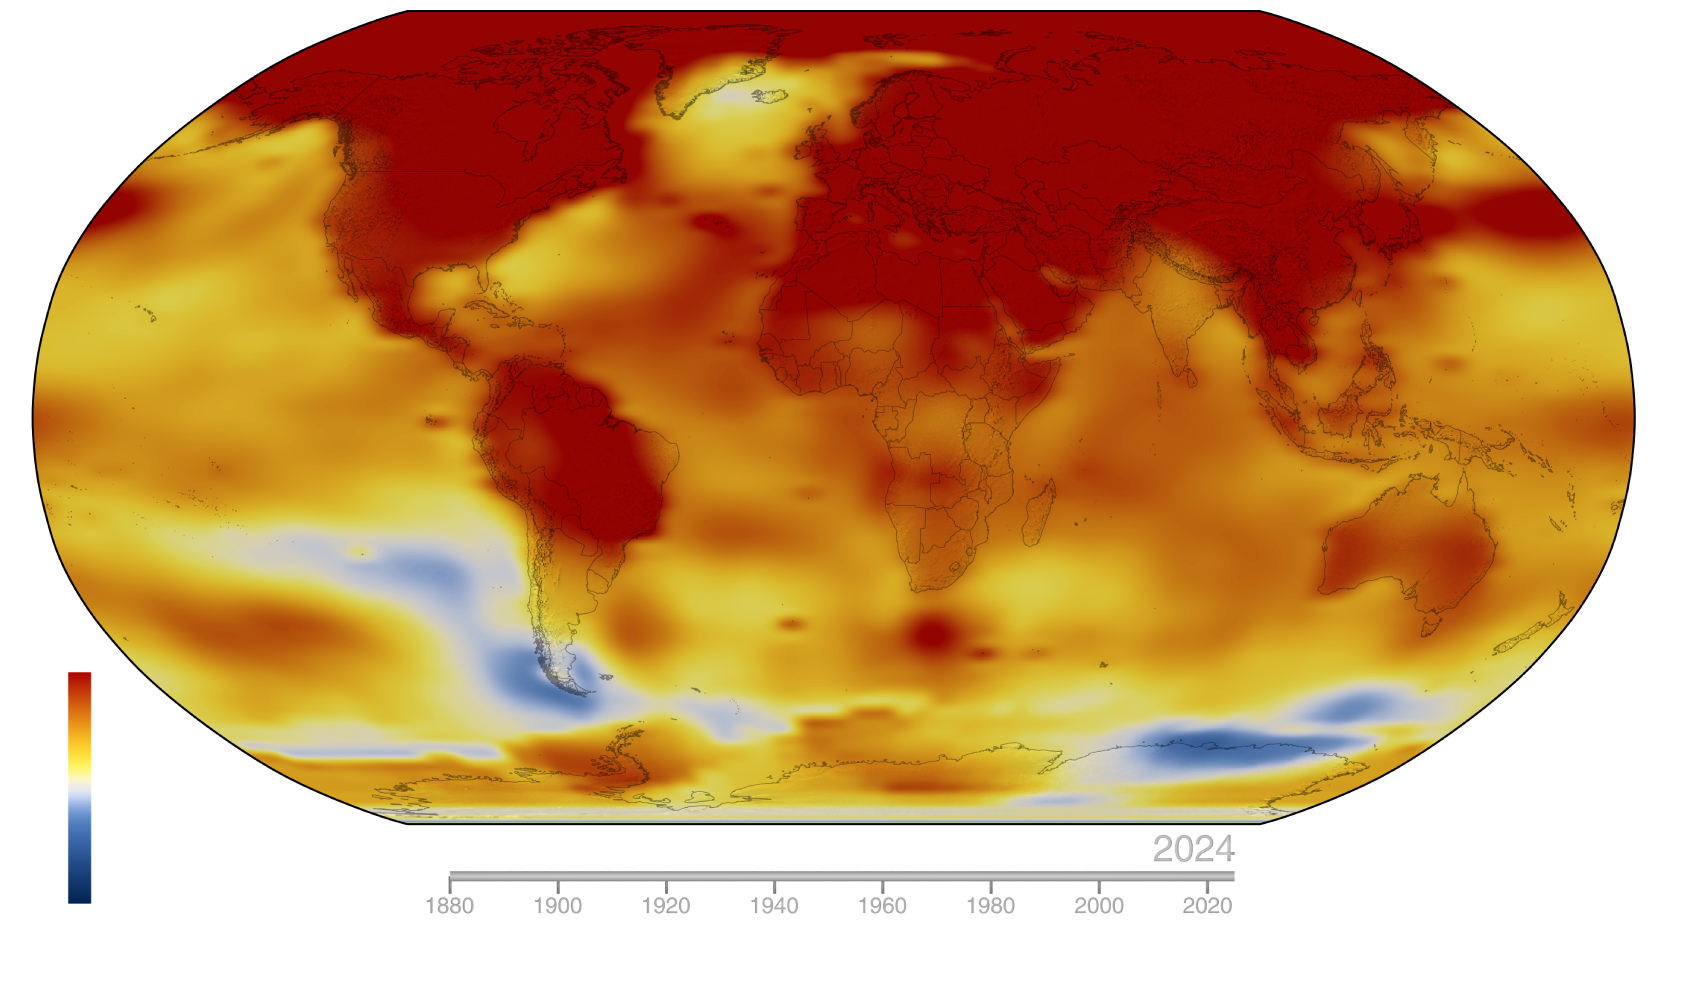
\includegraphics{2024-300dpi}\caption{Global Temperature 2024, source by NASA Earth Indicator. Available from https://science.nasa.gov/earth/explore/earth-indicators/
	global-temperature/\label{fig:NASA-Global-Temperature-2024}}
\end{figure}

The 1.5\textdegree C target is highly ambitious and is likely to  be surpassed
by 2025. Nevertheless, it remains significant as a benchmark for minimizing,
to the greatest extent possible, the impacts of natural disasters
that are exacerbated by climate change.\\
 Subsequently, we will present
numerical evidence illustrating how major natural disasters have become
increasingly frequent and intense over time, as a result of the evolving
impacts of climate change.\\
 Our data were retrieved from the\textit{
(EM-DAT) Emergency Events Database\cite{EM-DATA}},  
on 9 November 2025.\clearpage

From 1900 to 2025, a total of major events were recorded, around the
world categorized as follows \Tabref{Table-1-Hazards-1900--}

\begin{table}[H]
\begin{tabular}{|c|c|c|c|c|}
\hline
\textbf{\textcolor{blue}{Type of Hazards}} & \textbf{\textcolor{blue}{Years}} & \textbf{\textcolor{blue}{Years}} & \textbf{\textcolor{blue}{Years}} & \textbf{\textcolor{blue}{Years}}\tabularnewline
\hline
\hline
\textbf{Droughts} & \textbf{1900 - 1930} & \textbf{1931 - 1960} & \textbf{1961 - 1990} & \textbf{1991 - 2025}\tabularnewline
\hline
\textbf{Events} & 18 & 14 & 235 & 387\tabularnewline
\hline
\textbf{Human Casualties} & 6.048.400 & 3.450.000 & 3.186.981 & 26.723\tabularnewline
\hline
 &  &  &  & \tabularnewline
\hline
\textbf{Forest Fires} & \textbf{1900 - 1930} & \textbf{1931 - 1960} & \textbf{1961 - 1990} & \textbf{1991 - 2025}\tabularnewline
\hline
\textbf{Events} & 4 & 6 & 62 & 225\tabularnewline
\hline
\textbf{Human Casualties} & 1.176 & 332 & 500 & 2.039\tabularnewline
\hline
 &  &  &  & \tabularnewline
\hline
\textbf{Floods} & \textbf{1900 - 1930} & \textbf{1931 - 1960} & \textbf{1961 - 1990} & \textbf{1991 - 2025}\tabularnewline
\hline
\textbf{Events} & 27 & 116 & 983 & 3.881\tabularnewline
\hline
\textbf{Human Casualties} & 106.748 & 6.535.203 & 146.563 & 184.376\tabularnewline
\hline
 &  &  &  & \tabularnewline
\hline
\textbf{Landslide Wet} & \textbf{1900 - 1930} & \textbf{1931 - 1960} & \textbf{1961 - 1990} & \textbf{1991 - 2025}\tabularnewline
\hline
\textbf{Events} & 7 & 31 & 189 & 500\tabularnewline
\hline
\textbf{Human Casualties} & 539 & 20.720 & 18.928 & 25.247\tabularnewline
\hline
 &  &  &  & \tabularnewline
\hline
\textbf{Extreme Temperature} & \textbf{1900 - 1930} & \textbf{1931 - 1960} & \textbf{1961 - 1990} & \textbf{1991 - 2025}\tabularnewline
\hline
\textbf{Events} & No data & 10 & 73 & 560\tabularnewline
\hline
\textbf{Human Casualties} & No data & 3.189 & 8.994 & 353.849\tabularnewline
\hline
 &  &  &  & \tabularnewline
\hline
\textbf{Earthquakes} & \textbf{1900 - 1930} & \textbf{1931 - 1960} & \textbf{1961 - 1990} & \textbf{1991 - 2025}\tabularnewline
\hline
\textbf{Events} & 127 & 199 & 403 & 740\tabularnewline
\hline
\textbf{Human Casualties} & 619.013 & 374.020 & 568.013 & 623.195\tabularnewline
\hline
 &  &  &  & \tabularnewline
\hline
\textbf{Storms} & \textbf{1900 - 1930} & \textbf{1931 - 1960} & \textbf{1961 - 1990} & \textbf{1991 - 2025}\tabularnewline
\hline
\textbf{Events} & 76 & 248 & 1.136 & 2.286\tabularnewline
\hline
\textbf{Human Casualties} & 199.833 & 263.936 & 532.613 & 390.305\tabularnewline
\hline
 &  &  &  & \tabularnewline
\hline
\end{tabular}

\caption{Hazards 1900 - 2025.\label{tab:Table-1-Hazards-1900--}}

\end{table}



According to the available data, we conclude that natural disasters
have increased over the past 35 years when compared with the preceding
90 years. More specifically, there has been a rise in droughts, forest
fires, floods, landslides, extreme temperatures, earthquakes and storms.

\clearpage
\subsection{\textmd{The Dataset Employed }}
\vspace{-2em}
In this study, we utilized Historical Weather Data provided by Visual
Crossing \cite{Visual Crossing}, last accessed on
13 December 2025, which aggregates information from multiple authoritative
sources, including national meteorological services, global climate
models, and satellite observations. \\
Specifically, the data originate 
from verified governmental agencies such as NOAA, the German DWD, 
and the UK Met Office, as well as from certified private networks. 
This ensures the highest possible accuracy for each location.\\ 
Through continuously updated, high resolution models,
 Visual Crossing provides reliable information that supports informed 
 decision making regardless of the geographical area of interest.\\
 In order to gain access in the historical data, we first completed 
 the registration process. Subsequently,
by selecting data access, we defined the region of interest and the
desired date range. We then proceeded with the data retrieval process,
with a limit of 1,000 records per day in order to remain within the
free access tier. The overall procedure is straightforward, and the
only limitation encountered was the daily cap of 1,000 data points.

\subsection{\textmd{The Dataset Description}}
\vspace{-2em}
We downloaded historical meteorological data covering the period from
1995 to 2025, spanning approximately 30 years, to support the needs
of our climate change research. In addition, we selected regions across
different geographical latitudes and longitudes in order to obtain
a more comprehensive understanding of the areas most affected by the
global increase in temperature.\\
 The selected regions of interest are:
Congo, Saudi Arabia, Greece, Turkey, Reykjavik, Svalbard, and Cape
Town. The climatic data for all regions span the period from January
1, 1995, to December 13, 2025.\\
 Specifically, Turkey provides the most
complete dataset with 11,300 days of recordings, followed by Saudi
Arabia with 11,299 days, Svalbard with 11,297 days, Greece with 11,291
days, Congo with 11,202 days, Iceland with 11,140 days, and finally
Cape Town with 10,957 days. \\
All regions have consistent 30 columns
structure \tabref{Table-2-structure-columns}, 30+ years of data per
region, and multiple climate zones, such as: Mediterranean (Greece
\& Turkey), Arctic (Iceland Reykjavik \& Svalbard), Desert (Saudi
Arabia), Tropical (Congo), Temperate (Cape Town). The differences
in the number of data entries  due to gaps (missing values) present
in the records obtained from Visual Crossing, which did not affect
our results.

\begin{table}[H]
	\centering
\begin{tabular}{|c|c|c|}
\hline
\textbf{\textcolor{blue}{Number}} & \textbf{\textcolor{blue}{Data}} & \textbf{\textcolor{blue}{Values}} \tabularnewline
\hline
\hline
1 & Temperature max (Fahrenheit) & \textdegree F \tabularnewline
\hline
2 & Temperature min (Fahrenheit) & \textdegree F \tabularnewline
\hline
3 & Feels like max (Fahrenheit) & \textdegree F \tabularnewline
\hline
4 & Feels like min (Fahrenheit) & \textdegree F \tabularnewline
\hline
5 & Feels like (Fahrenheit) & \textdegree F \tabularnewline
\hline
6 & Dew & \textdegree F \tabularnewline
\hline
7 & Humidity & \% \tabularnewline
\hline
8 & Precipitation & in \tabularnewline
\hline
9 & Precipitation prob &  \% \tabularnewline
\hline
10 & Precipitation cover & \% \tabularnewline
\hline
11 & Precipitation type & Type(s) \tabularnewline
\hline
12 & Snow & in \tabularnewline
\hline
13 & Snow depth & in \tabularnewline
\hline
14 & Windgust & mph \tabularnewline
\hline
15 & Wind speed & mph \tabularnewline
\hline
16 & Wind dir & ($^\circ$) \tabularnewline
\hline
17 & Sea level pressure & mb\tabularnewline
\hline
18 & Cloud cover & \% \tabularnewline
\hline
19 & Visibility & mi \tabularnewline
\hline
20 & Solar radiation & $(W/m^2)$ \tabularnewline
\hline
21 & Solar energy & $(MJ/m^2)$ \tabularnewline
\hline
22 & Uvindex &  (0 - 10) \tabularnewline
\hline
23 & Severe risk & (0 - 100) \tabularnewline
\hline
24 & Moon phase & (0 - 1)\tabularnewline
\hline
25 & Temp max (Celsius) & \textdegree C \tabularnewline
\hline
26 & Temp min (Celsius) & \textdegree C \tabularnewline
\hline
27 & Year &  (1995 - 2025) \tabularnewline
\hline
28 & Month &  (0 - 12)\tabularnewline
\hline
29 & Day & (1 - 31) \tabularnewline
\hline
30 & Class & (0 / 1) \tabularnewline
\hline
 & & \tabularnewline
\hline
\end{tabular}\caption{Table structure columns climate data\label{tab:Table-2-structure-columns}}
\end{table}

In summary, we report the maximum and minimum values of the average
temperature for each region. For Greece, the highest recorded value
was 36\textdegree C (96.8\textdegree F) on July 21, 2011, while the lowest was \textminus 26.33\textdegree C
(-15.4\textdegree F) on January 27, 2003. In Turkey, the maximum temperature
was recorded on July 30, 2000, at 41.05\textdegree C (105.9\textdegree F), while the minimum
reached \textminus 22.94\textdegree C (\textminus 9.3\textdegree F) on February 16, 2006.
In Saudi Arabia, the maximum temperature approached 48.2\textdegree C (118.9\textdegree F)
on May 30, 2021, while the minimum reached \textminus 2.05\textdegree C (28.3\textdegree F)
on January 17, 2008.\\ In Cape Town, the maximum temperature reached
42\textdegree C (107.6\textdegree F) on February 3, 2015, while the minimum was 0.05\textdegree C (32.1\textdegree F),
a value that occurred seven times: twice in July 1996, twice in 2000,
and once in 2001, 2002, and 2003. In Reykjavik, Iceland, the maximum
temperature was 25.7\textdegree C (78.3\textdegree F) on July 30, 2008, while the minimum
reached \textminus 14.3\textdegree C (6.2\textdegree F) on July 3, 1998.\\
 In Congo, the maximum
temperature reached 39.05\textdegree C (102.3\textdegree F) on February 22, 1995, while
the minimum was 12.5\textdegree C (54.6\textdegree F) on June 7, 2012. In Svalbard, the
maximum temperature reached 33.38\textdegree C (92.1\textdegree F) on July 20, 2022, while
the minimum was \textminus 15.11\textdegree C (4.8\textdegree F) on January 5, 2003.

From these observations, it is striking that Greece recorded the lowest
temperature \textminus 26.33\textdegree C (-15.4\textdegree F), followed by Turkey \textminus 22.94\textdegree C
(\textminus 9.3\textdegree F) compared to regions located within the Arctic Circle,
while the highest value was, as expected, observed in Saudi Arabia,
a country characterized by a desert climate.\\
 In addition, over the
period from January 1, 1995, to December 8, 2025, all seven regions
under investigation exhibited an increase in mean temperature, albeit
with varying magnitudes.\\
 Turkey recorded the highest rise at 1.92\textdegree C
(3.46\textdegree F), followed by Reykjavik with 1.41\textdegree C (2.54\textdegree F) and Greece with
1.22\textdegree C (2.20\textdegree F). More moderate increases were observed in Svalbard
(0.93\textdegree C; 1.67\textdegree F), Cape Town (0.81\textdegree C; 1.46\textdegree F), and Saudi Arabia (0.79\textdegree C;
1.42\textdegree F). Congo displayed the smallest change, with only 0.10\textdegree C (0.18\textdegree F).
These findings highlight both regional disparities and the broader
trend of warming consistent with the impacts of climate change \Tabref{Table-3-Mean-Temperature-increased-1995-2025}.

\begin{table}[H]
		\centering
\begin{tabular}{|c|c|c|}
\hline
\textbf{\textcolor{blue}{Number}} & \textbf{\textcolor{blue}{Region}} & \textbf{\textcolor{blue}{Mean Temperature increased}}\tabularnewline
\hline
\hline
1 & Turkey & 1.92\textsuperscript{o}C (3.46\textsuperscript{o}F)\tabularnewline
\hline
2 & Reykjavik & 1.41\textsuperscript{o}C (2.54\textsuperscript{o}F)\tabularnewline
\hline
3 & Greece & 1.22\textsuperscript{o}C (2.20\textsuperscript{o}F)\tabularnewline
\hline
4 & Svalbard & 0.93\textsuperscript{o}C (1.67\textsuperscript{o}F)\tabularnewline
\hline
5 & Cape Town & 0.81\textsuperscript{o}C (1.46\textsuperscript{o}F)\tabularnewline
\hline
6 & Saudi Arabia & 0.79\textsuperscript{o}C (1.42\textsuperscript{o}F)\tabularnewline
\hline
7 & Congo & 0.10\textsuperscript{o}C (0.18\textsuperscript{o}F)\tabularnewline
\hline
\end{tabular}

\caption{Mean Temperature increased 1995 2025\label{tab:Table-3-Mean-Temperature-increased-1995-2025}}

\end{table}

After examining our dataset and identifying the variations in temperature
across the seven regions under study, we proceeded with the classification
of temperatures. To achieve this, the classification scheme required
adaptation for each region individually. Specifically, we calculated
the mean temperature for each region using the first five years of
data, namely from 1995 to 2000. This mean value was employed as the
baseline. Temperatures that were either lower or higher by up to 1 Celsius
relative to this baseline were assigned to Class 0,
whereas temperatures exceeding the baseline by more than 1.1 
were assigned to Class 1 \Tabref{Table-4-Region-Baseline-Class}.

 {The formulation of the problem may appear simplified through the use of a binary classification scheme. However, this choice is directly aligned with the central issues of climate change, particularly global temperature increase. In recent years, major environmental institutions and international climate agreements (as discussed in  Introduction) have repeatedly emphasized the critical need for countries to limit global warming and prevent the mean temperature rise from exceeding 1.5\textsuperscript{o}C.}
{Therefore, adopting a binary classification framework is intentional and scientifically meaningful. While a difference of one degree may seem small from a numerical perspective, it represents a substantial and highly consequential threshold for planetary sustainability. In this context, the classification captures a climate - critical distinction rather than a trivial fluctuation.}

The definition of the two classes was based on the environmental considerations
discussed in our introduction, aligned with the Paris Agreement and
the 1.5\textdegree C climate target, as well as on our data-driven analyses
and the class balance that we were able to achieve. Similarly, the
temporal span of our dataset was selected to align with the climatological
milestones commonly used to characterize the progression of climate
change.\\
 For this reason, we adopted the period 1995--2025 as the
analysis window across the different climatic regions. Furthermore,
the definition of our classes was made with careful consideration,
and the first class explicitly includes negative temperature anomalies,
as it encompasses all temperature values from below zero up to +1\textdegree C.

\begin{table}[H]

\begin{tabular}{|c|c|c|c|c|}
\hline
\textbf{\textcolor{blue}{Number}} & \textbf{\textcolor{blue}{Region}} & \textbf{\textcolor{blue}{Baseline for Class}} & \textbf{\textcolor{blue}{Class 0 (total data)}} & \textbf{\textcolor{blue}{Class 1 (total data)}}\tabularnewline
\hline
\hline
1 & Turkey & 11.32 & 5.549 & 5.752\tabularnewline
\hline
2 & Reykjavik & 4.715 & 5.681 & 5.620\tabularnewline
\hline
3 & Greece & 9.06833333 & 5.629 & 5.662\tabularnewline
\hline
4 & Svalbard & 8.96666667 & 5.957 & 5.345\tabularnewline
\hline
5 & Cape Town & 16.605 & 6.118 & 5.183\tabularnewline
\hline
6 & Saudi Arabia & 26.88666667 & 5.531 & 5.767\tabularnewline
\hline
7 & Congo & 25.646667 & 7.536 & 3.666\tabularnewline
\hline
\end{tabular}

\caption{Region Baseline Class 1995 2000\label{tab:Table-4-Region-Baseline-Class}}

\end{table}

The rationale for selecting the initial five-year period was to establish
a reference point unaffected by the extreme temperature fluctuations
associated with climate change, given that our dataset spans from
1995 to 2025. This approach ensured that the classification was grounded
in a stable climatic baseline, thereby enhancing the reliability of
subsequent analysis.\\
{Finally, we note that regarding temporal leakage, we clarify that the class labels were generated manually using historical temperature data only, and no future information was used at any stage of preprocessing. At the same time, we note in the final part of the conclusions section the relevant limitations concerning the need for time - series - aware evaluation strategies.}


\subsection{\textmd{The proposed method\label{subsec:The-proposed-method}}}

The current work proposed the incorporation of a method that constructs
classification rules, initially proposed in \textit{\cite{Tsoulos 2020}.}
Furthermore, this method was implemented as a software recently \textit{\cite{Anastasopoulos 2021}.}
The published software GENCLASS is an open\nobreakdash-source software
tool, publicly available on GitHub \cite{GitHub},where detailed installation 
instructions and usage examples are provided.
The software is implemented in ANSI C++ and supports Python\nobreakdash-formatted
rule output.\\
 Its execution is controlled through a set of command\nobreakdash-line
parameters that define all key aspects of the method, including the
number of chromosomes, number of generations, mutation rate, and other
evolutionary settings. The implementation relies on OpenMP for multicore
parallelization and uses Grammatical Evolution with a BNF grammar
to generate human\nobreakdash-readable classification rules.

The objective of the proposed method is to achieve high-accuracy classification
of daily climate observations into temperature-change categories,
while preserving interpretability through explicit rules.

{At this point, before proceeding to the detailed description of the procedures, we provide a two - part summary of our study. The first part of our work involved the statistical analysis of the dataset, which produced the temperature increase percentages for the regions of interest and enabled the definition of two classes. The second and main part of the current study focuses on validating these results using various machine - learning techniques.}

{The two classes (0, 1) were not generated by the Genetic Algorithm. They were defined by us prior to the experiments, using explicit temperature baselines:
\begin{itemize}
	\item Class 0: increase up to 1\textsuperscript{o}C
	\item Class 1: increase above 1.1\textsuperscript{o}C
	\end{itemize}}

{These initial steps were performed manually in Excel before converting the dataset to CSV. The data were then transformed into a format compatible with the Optimus/GENCLASS framework, as described in the current section.
Therefore, the Genetic Algorithm does not operate as a black box: its fitness function evaluates how well the evolved rules classify these scientifically defined categories based on the meteorological parameters.}

Grammatical Evolution produces concrete if-then programs over the available features,
making nonlinear relationships transparent and directly inspectable.
Empirically, GENCLASS demonstrates better performance over the considered
baselines  across all regions, achieving the
lowest mean classification error (AVERAGE 1.66\%) and consistently
high precision/recall. \\
Although strong deep sequence models for climate
time series exist (e.g., LSTM/CDLSTM), the present study focuses on
interpretable rule-induction and benchmarking against established
conventional learners; a comprehensive comparison against deep sequence
architectures under strictly time-ordered evaluation protocols is
a natural extension for future work.

The proposed model, through the use of BNF grammar and Grammatical
Evolution, is able to construct rules that exploit only the necessary
features of the dataset under study. In this way, the model becomes
more flexible and faster in decision-making, even when dealing with
large datasets. Moreover, since it relies solely on the essential
information for rule generation, it may exhibit better generalization
capabilities compared to other machine learning models.\\
 The underlying
grammar for this method is provided in \Figref{The-underlying-grammar-method}. In this grammar the constant $D$ has the value $D=30$ since the number of features for the used data is set 30, as shown in Table \ref{tab:Table-2-structure-columns}. For example, the variable X2 encodes the minimum temperature etc.
\begin{figure}[H]
	\centering
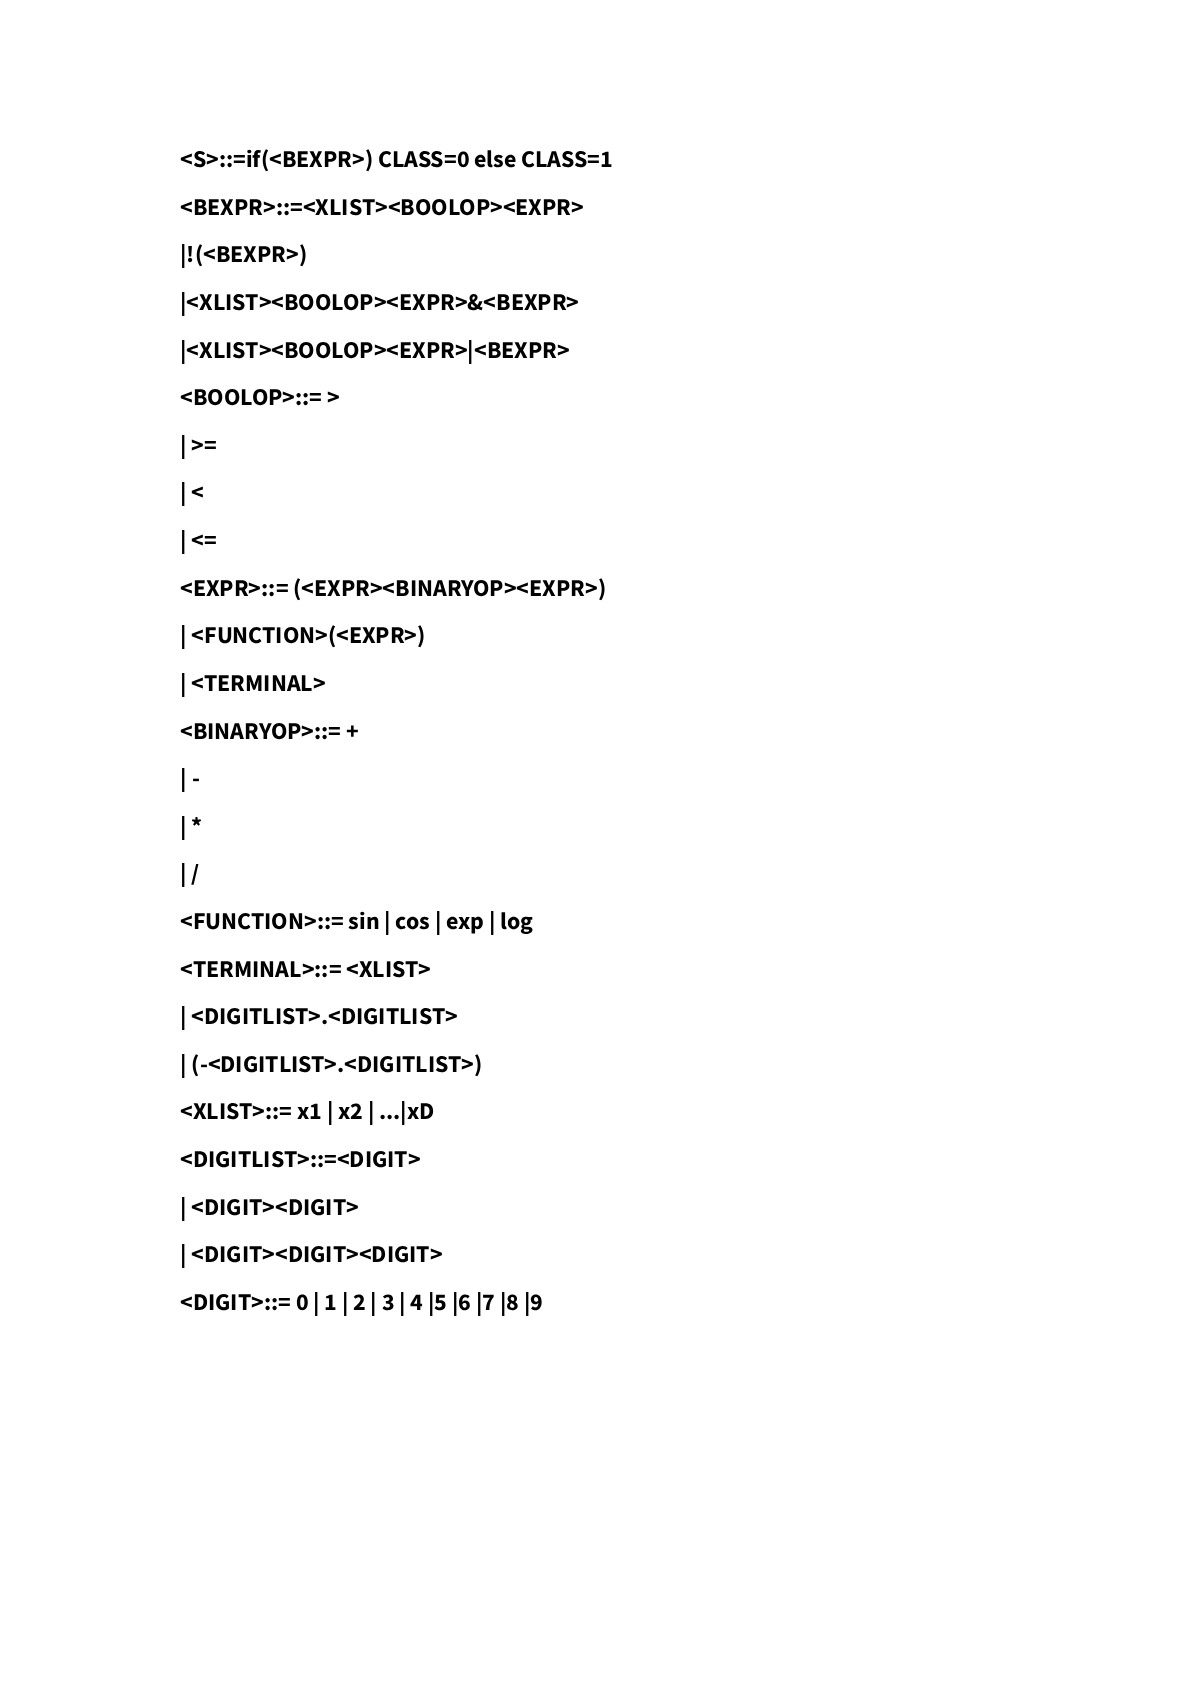
\includegraphics[scale=0.7]{grammar_method(fig4)}
\caption{The underlying grammar for the method that produces classification
programs using Grammatical Evolution\label{fig:The-underlying-grammar-method}}
\end{figure}
\clearpage
The steps for this method have as follows:
\begin{enumerate}
\item Initialization step.
\begin{enumerate}
\item Set with \textit{\textcolor{blue}{N\textsubscript{c}}} the number
of chromosomes and with \textit{\textcolor{blue}{N\textsubscript{g}}}
the number of allowed generations.
\item Set the selection rate \textit{\textcolor{blue}{p\textsubscript{s}
}}and the mutation rate \textit{\textcolor{blue}{p\textsubscript{m}.}}
\item Initialize each chromosome$c_{i},\ i=1,\ldots,N_{c}$ as a set of
randomly selected integers.
\item Set $k=0$, that defines the generation counter.
\end{enumerate}
\vspace{2em}
\item Fitness calculation step.
\begin{enumerate}
\item For i = 1, . . . , \textit{\textcolor{blue}{N\textsubscript{c}}}
do
\vspace{2em}
\begin{enumerate}
\item Construct with the procedure of Grammatical evolution and the incorporation
of the BNF grammar of \Figref{The-underlying-grammar-method} a classification
program $G_{i}$ that corresponds to the elements of chromosome $c_{i}$.
\item Calculate the associated fitness$f_{i}$ value as
\begin{equation}
f_{i}=\sum_{j=1}^{M}\left(G_{i}\left(x_{j}\right)-t_{j}\right)^{2}
\end{equation}
The set $T=\left\{ \left(x_{1},t_{1}\right),\left(x_{2},t_{2}\right),\ldots,\left(x_{M},t_{M}\right)\right\} $denotes
the training set of the objective problem, where the vectors$x_{i}$
stand for the input patterns and each value $t_{i}$ represents the actual
output for pattern $x_{i}$. \\
The proposed method in practice uses
the mean classification error on the training set as the fitness measure,
since the output of the produced model is one of the available categories
of the dataset under study.
\end{enumerate}
\item End For \clearpage 
\end{enumerate}
\vspace{1em}
\item Application of Genetic Operations.
\begin{enumerate}
	\vspace{-4em}
\item Selection procedure. The remaining are substituted by chromosomes
produced during crossover and mutation. \\
The top $p_{s}\times N_{c}$
chromosomes are directly carried over to the next generation, while
the rest are replaced by chromosomes generated through crossover and
mutation.
\item Crossover procedure. This procedure produces new chromosomes from
the current population.
 For every pair $\left(c_{1},c_{2}\right)$
of new chromosomes two chromosomes denoted as $p_{1}$ and $p_{2}$
are selected from the current population using tournament selection.
The production of $\left(c_{1},c_{2}\right)$ will be performed using
one - point crossover \textit{\cite{Poli 1998}}. 
\vspace{-5em}
An example of this
procedure is outlined in \Figref{A-graphical-example}.
\vspace{3.6em}
\begin{figure} [H]
	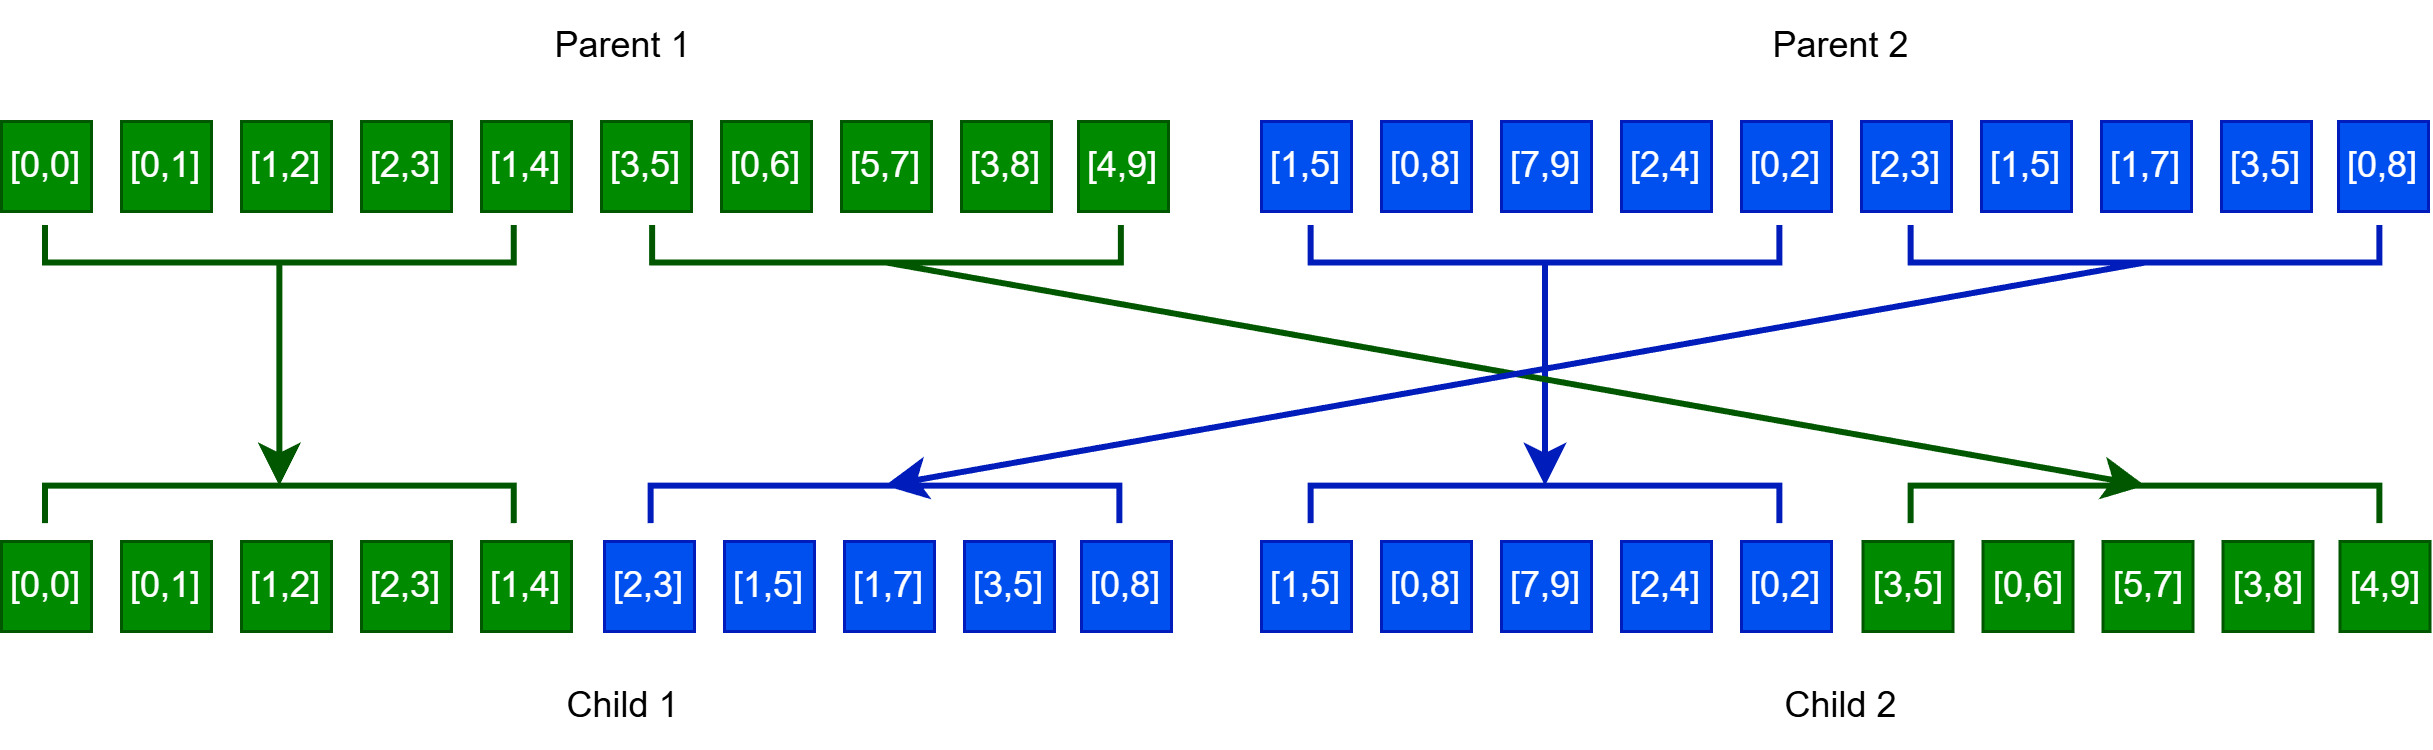
\includegraphics[scale=0.55]{crossover(fig5)}
		\centering	
	\caption{A graphical example of the one - point crossover.\label{fig:A-graphical-example}}
\end{figure}
\vspace{2em}
\item Mutation procedure. Draw a random number $r\le1$ for each element
of every chromosome. Alter randomly this element when $r\le p_{m}$.
The mutation procedure is depicted as a flowchart in \Figref{The-flowchart-of}
\end{enumerate}

\begin{figure}[H]
	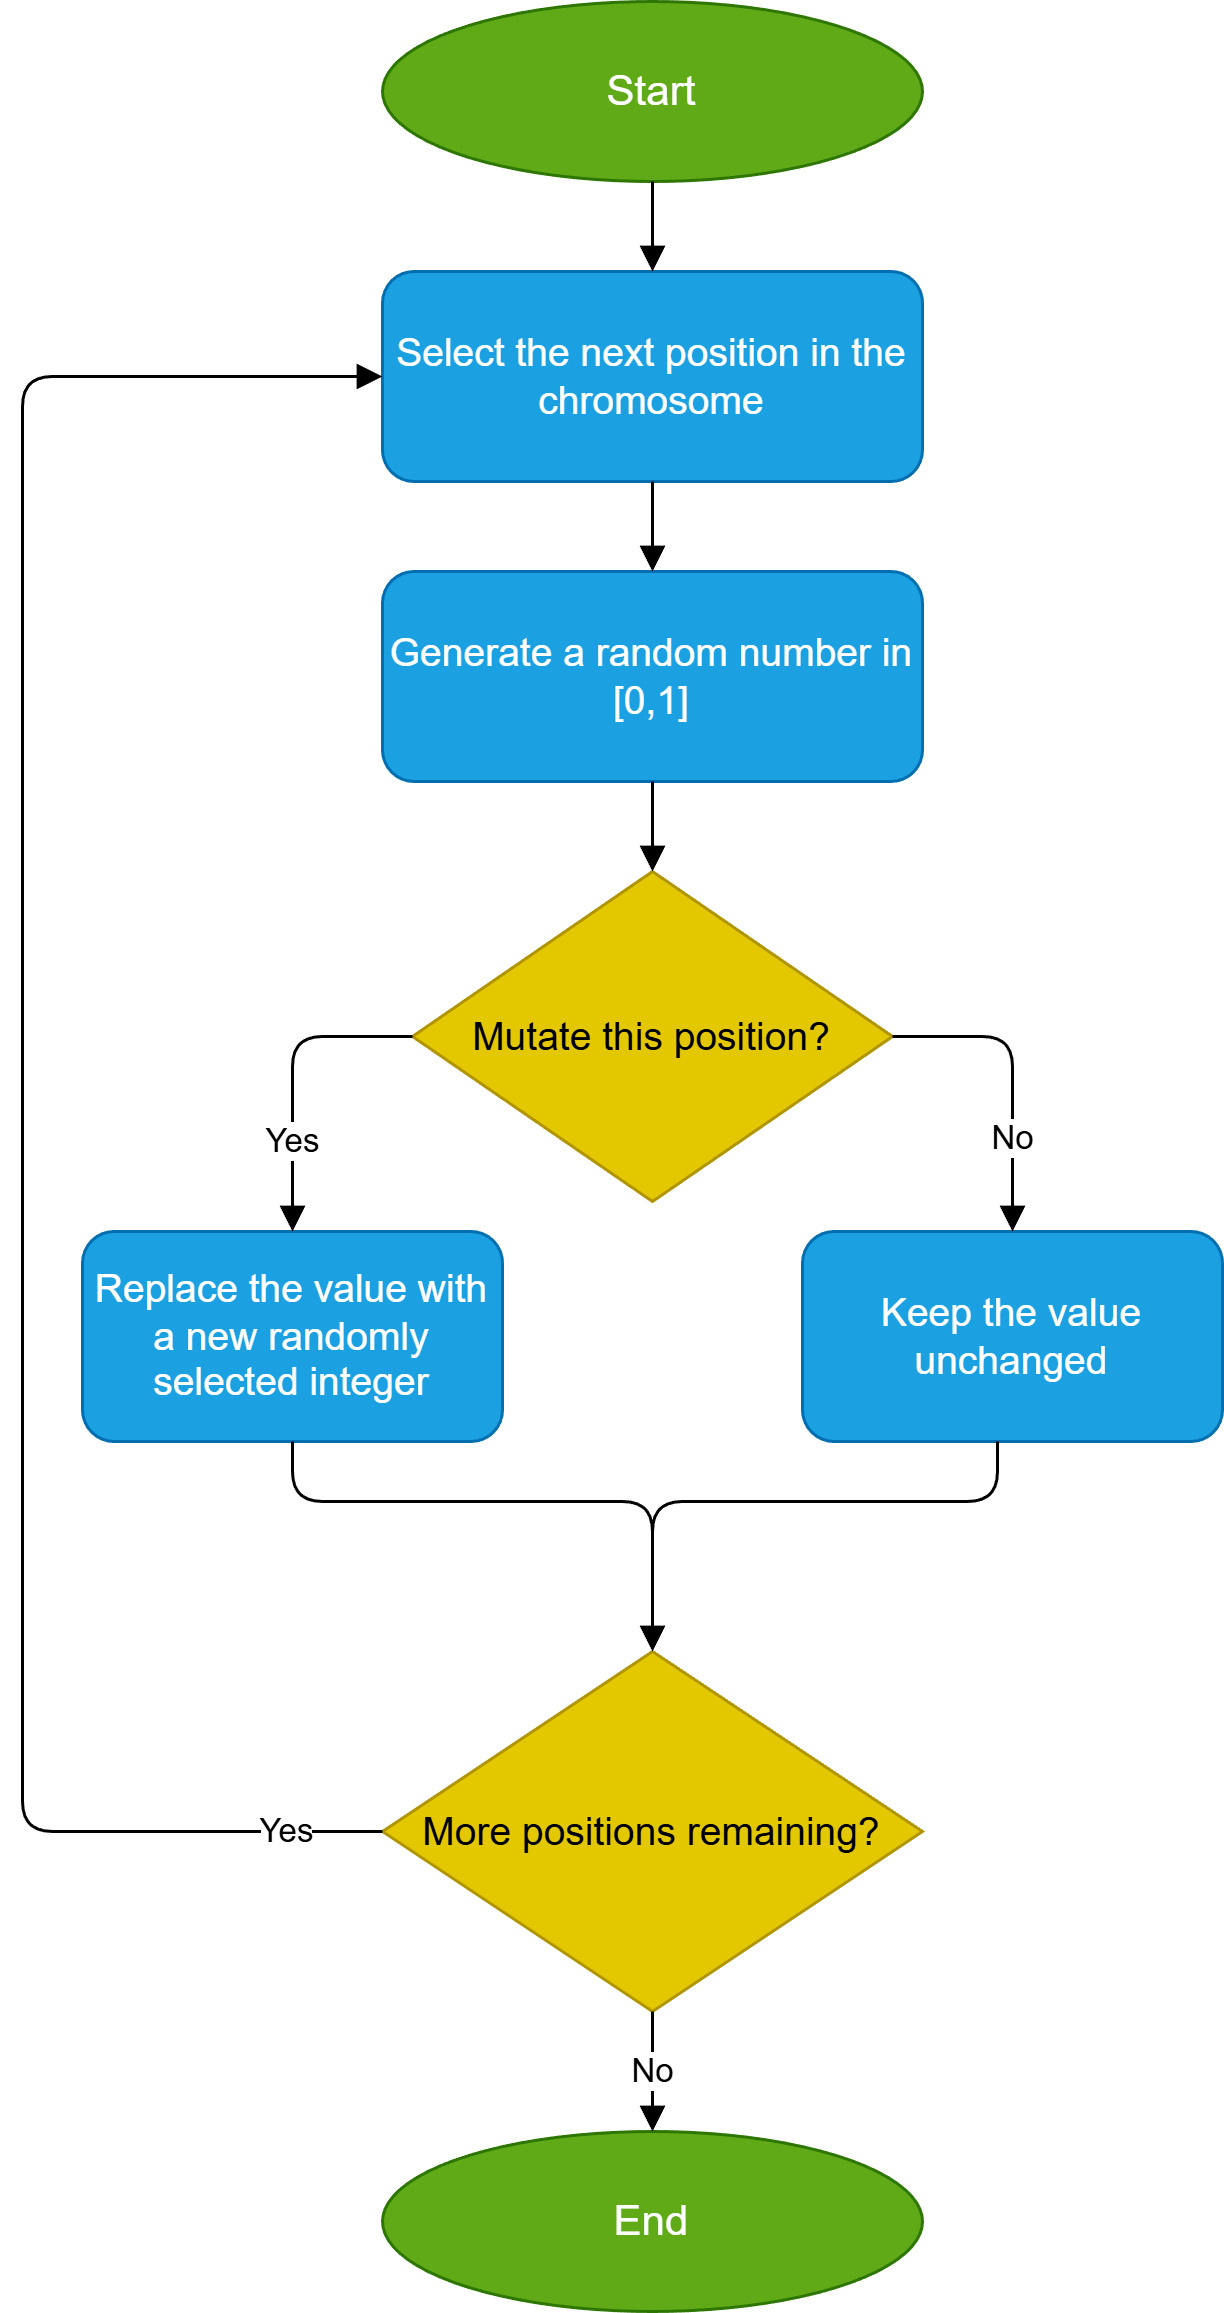
\includegraphics[scale=0.7]{mutation_flowchart}
	\centering	
	\caption{The flowchart of the mutation procedure\label{fig:The-flowchart-of}}
\end{figure}



\item Termination check step.

\begin{enumerate}
\item Set $k=k+1$
\item If $k<N_{g}$ then go to Fitness calculation step else go to Testing
step.
\end{enumerate}

	
\item Testing step.

\begin{enumerate}
\item Get the best chromosome $c^{*}$ of the population with the lowest
fitness value and create the corresponding classification program
$G^{*}$.
\item Apply the classification program to the test set of the objective
problem and calculate the corresponding test error.
\end{enumerate}
\end{enumerate}\clearpage
The overall procedure is graphically outlined in \Figref{The-flowchart-of-1}.
\begin{figure}[H]
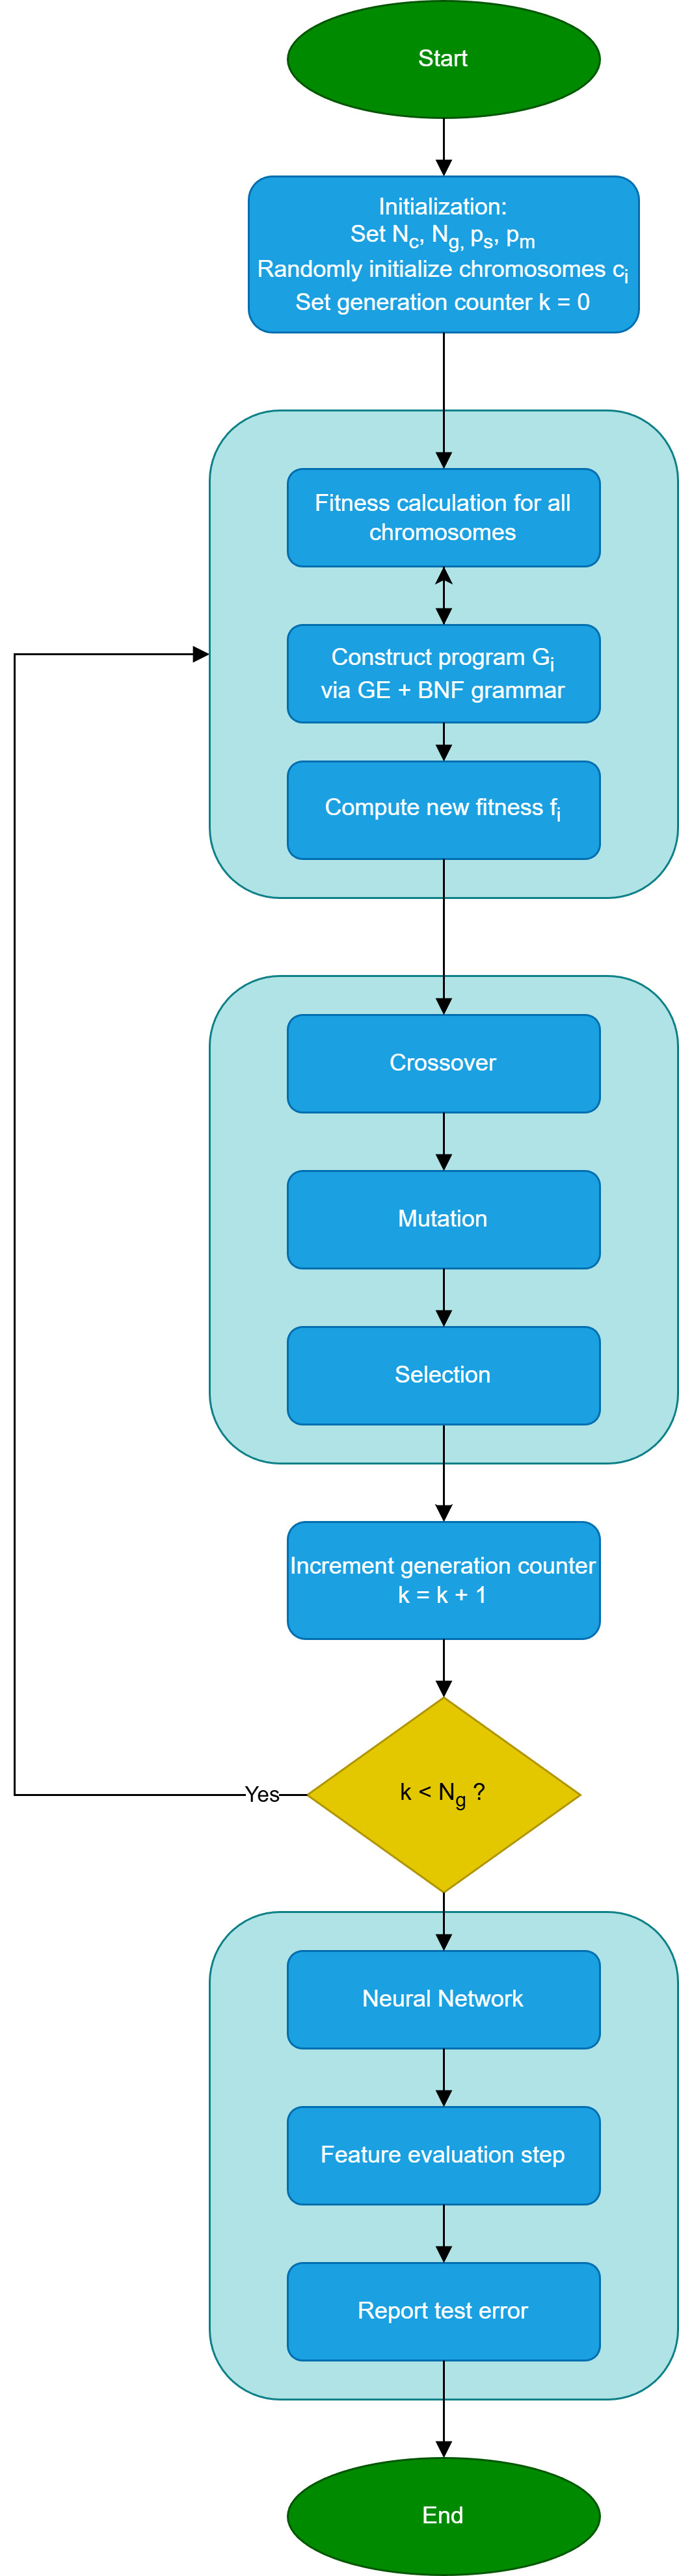
\includegraphics[scale=0.6]{genclass_flowchart(fig7)}
\centering
\caption{The flowchart of the proposed method\label{fig:The-flowchart-of-1}}
\end{figure}


\clearpage
\section{Results\label{sec:Results}}
The software used in the experiments was coded in C++ programming
language and the freely available software Optimus \textit{\cite{Tsoulos 2025},}
 with last accessed on 25 December 2025, was incorporated for the optimization methods.
The experimental results were validated using the ten - fold cross
validation procedure and all the experiments were executed on a Debian
Linux machine with 128GB of ram. The values for the experimental parameters
are outlined in Table \ref{tabTable-5-:Experimental-settings}.\\
{At this point, before proceeding to the detailed description, we outline clarifications concerning the validation strategy of the results.  The validation process begins with the use of historical, day by day climate observations from 1995 to 2025. Each time step corresponds to a single day, and the class label (0 or 1) was assigned solely on the basis of each day mean temperature. This ensures that the class procedure relies strictly on past information, and therefore no temporal leakage occurs during preprocessing.}
{Subsequently, the defined classes were validated using machine learning algorithms and the GENCLASS evolutionary framework. Nevertheless, as also noted Conclusions section, we acknowledge that random cross validation does not explicitly preserve temporal ordering and may introduce limitations when dealing with time dependent climate data. For this reason, we explicitly highlight the need for time-series-aware evaluation protocols as an important consideration for future extensions of this work.}

\begin{table}[H]
	\centering
\begin{tabular}{|c|c|c|}
	
\hline
\textbf{\textcolor{blue}{PARAMETER}} & \textbf{\textcolor{blue}{PURPOSE}} & \textbf{\textcolor{blue}{VALUE}}\tabularnewline
\hline
\hline
\textit{\textcolor{blue}{N\textsubscript{c}}} & Number of Chromosomes & 500\tabularnewline
\hline
\textit{\textcolor{blue}{N\textsubscript{g}}} & Maximum number of generations & 1.000\tabularnewline
\hline
\textit{\textcolor{blue}{P\textsubscript{s}}} & Selection rate & 0.10\tabularnewline
\hline
\textit{\textcolor{blue}{P\textsubscript{m}}} & Mutation rate & 0.05\tabularnewline
\hline
\textit{\textcolor{blue}{H}} & Number or weights for neural network & 10\tabularnewline
\hline
\end{tabular}

\caption{Experimental settings\label{tabTable-5-:Experimental-settings}}
\end{table}

The \Tabref{Table-6-Experimental-results-on} summarizes the experimental
results on datasets derived from various areas using a series of machine
learning methods. The following notation is used in the experimental
tables:
\begin{enumerate}
\item The column dataset denotes the objective dataset.
\item The column MLP represents the results derived from the application
of an artificial neural network with 10 processing nodes. This network
was trained using the BFGS variant of Powell \textit{\cite{M.J.D Powell 1989}}
as the training method.
\item The column The column RBF denotes the application of a Radial Basis
Function (RBF) network\textit{\cite{J. Park 1991,G.A. Montazer 2018}
}to the related dataset. This network has 10 processing nodes.
\item The column SVM represents the application of the SVM method, using
the implementation provided in the freely available library of LibSvm
\textit{\cite{Chang 2011}.}
\item The column NNC stands for the usage of the Neural Network Construction
method, initially described in \textit{\cite{Tsoulos 2008}}. The
parameters used in the genetic algorithm for the NNC model are the
same as in the case of the GENCLASS model.
\item The column XGBOOST denotes the usage of the gradient boost technique \textit{\cite{xgboost}}.
\item The column BAYESNN represents the incorporation of  the Bayesian optimizer as implemented in the BayesOpt  library \textit{\cite{bayesnn}} in order to  train a neural network with $H=10$ computing nodes.
\item The column DNN represents the usage of  a deep neural network, as implemented in the Tiny Dnn library freely available from  \url{https://github.com/tiny-dnn/tiny-dnn}. The network was trained using the  AdaGrad method \textit{\cite{adagrad}}.
\item The column GENCLASS indicates the incorporation of the proposed method
for construction of classification rules.
\item The row average represents the average classification error for all
used datasets.
\end{enumerate}
 \Tabref{Table-6-Experimental-results-on} reports the percentage
classification error obtained by five machine learning models (MLP,
RBF, SVM, NNC, and the proposed GENCLASS) across seven region-specific
climate-zone datasets (CAPETOWN, GREECE, ICELAND, CONGO, ARABIA, SVALBARD,
TURKEY). 

Since the entries are error percentages, lower values indicate
higher classification accuracy, while the final row (AVERAGE) summarizes
the mean error over all datasets. The dominant outcome is the consistent
superiority of GENCLASS, which achieves the lowest error on every
dataset and the best overall average (1.66\%).\\
 Importantly, this performance
should be interpreted in light of the strong geographical and environmental
heterogeneity represented by the selected regions, spanning a wide
range of latitudes and longitudes and encompassing markedly different
physical settings (coastal versus inland areas, mountainous terrain,
forests, deserts, glaciers/sea ice, and distinct hemispheric seasonality).
Such factors affect local temperature dynamics, variability, and seasonality
and therefore shape the complexity of the classification patterns
that each model must learn.\\
 For instance, CONGO lies close to the
Equator (approximately within a few degrees north and south of $0^\circ$
latitude, primarily at eastern longitudes in Central Africa) and is
characterized by extensive tropical rainforest cover and high atmospheric
moisture. \\
In this dataset,\Tabref{Table-6-Experimental-results-on}
shows the highest errors for most methods and also the largest GENCLASS
error (4.84\%), suggesting a comparatively more challenging classification
structure, plausibly due to weaker temperature seasonality and stronger
interactions with humidity and cloud-related processes.\\
 In contrast,
ARABIA (roughly $16^\circ$-$32^\circ$N at eastern longitudes in Western Asia) is
dominated by hot desert conditions, where land-surface properties,
low cloudiness, and persistent aridity often yield clearer and more
repeatable temperature-related signatures, accordingly, GENCLASS attains
a very low error (0.73\%) and NNC also performs strongly.\\
 In the Mediterranean/subtropical
band, GREECE combines strong maritime
influence, extensive coastline and island geography, and pronounced
mountainous terrain, all of which introduce microclimatic variability,
nevertheless, GENCLASS remains highly accurate (0.85\%), indicating
robust handling of nonlinear interactions linked to elevation, coastal
effects, and seasonal transitions typical of Mediterranean climates.\\
TURKEY  is even more heterogeneous,
with coastal zones influenced by surrounding seas and inland plateaus
and mountain ranges exhibiting more continental conditions, despite
this diversity, GENCLASS again yields the smallest error (0.63\%),
whereas conventional baselines such as MLP and SVM show substantially
larger errors.\\
 At higher latitudes, ICELAND
is shaped by oceanic
forcing, strong winds, glaciers, and complex volcanic topography,
which can increase meteorological variability.\\
 Still, GENCLASS keeps
the error relatively low (2.47\%) compared with the other methods.
SVALBARD 
represents an Arctic archipelago with extensive glaciation/sea-ice
influence and extreme photoperiodicity (polar night and midnight sun),
conditions that can produce strong seasonal contrasts and circulation-driven
variability, nevertheless, GENCLASS remains the most accurate method
(1.11\%), with NNC as the next best performer.\\
 Finally, CAPETOWN 
lies in the Southern Hemisphere and is typically described
by a Mediterranean-type regime with strong coastal forcing and nearby
mountainous relief that modulates winds and temperature variability,
here too GENCLASS attains the lowest error (0.97\%).\\
 The AVERAGE row
confirms that, when aggregating across all these diverse geographic
coordinates and environmental contexts, GENCLASS provides the most
reliable generalization with the smallest mean error, while NNC consistently
ranks second.\\
 Overall, the \Tabref{Table-6-Experimental-results-on}
supports not only that GENCLASS is more accurate, but also that it
generalizes effectively across datasets derived from regions with
fundamentally different latitude--longitude positioning and physical
environments, suggesting improved capacity to capture nonlinear relationships
and interactions induced by topography, land cover (forest/desert/ice),
proximity to oceans, and regional seasonality.
\begin{table}[H]
	\centering
	\footnotesize
\begin{tabular}{|c|c|c|c|c|c|c|c|c|}
\hline
\textbf{\textcolor{blue}{DATASET}} & \textbf{\textcolor{blue}{MLP}} & \textbf{\textcolor{blue}{RBF}} & \textbf{\textcolor{blue}{SVM}} & \textbf{\textcolor{blue}{NNC}} &
\textbf{\textcolor{blue}{XGBOOST}} &
\textbf{\textcolor{blue}{BAYESNN}} &
\textbf{\textcolor{blue}{DNN}} &
\textbf{\textcolor{blue}{GENCLASS}}\tabularnewline
\hline
\hline
\textbf{Cape Town} & 14.89\% & 12.43\% & 17.18\% & 2.00\% &
9.18\% & 13.43\%&14.12\% &
0.97\%\tabularnewline
\hline
\textbf{Greece} & 38.10\% & 4.34\% & 50.61\% & 6.15\% &
0.74\% & 6.33\% & 2.64\% &
0.85\%\tabularnewline
\hline
\textbf{Iceland} & 36.87\% & 7.09\% & 49.79\% & 6.33\% &
2.90\% & 10.25\% & 5.66\% &
2.47\%\tabularnewline
\hline
\textbf{Congo} & 26.52\% & 30.16\% & 32.71\% & 13.75\% &
32.72\% & 24.21\% & 30.35\% &
4.84\%\tabularnewline
\hline
\textbf{Arabia} & 41.63\% & 7.62\% & 48.94\% & 4.91\% &
0.37\% & 4.86\% & 1.28\% &
0.73\%\tabularnewline
\hline
\textbf{Svalbard} & 27.56\% & 23.30\% & 47.22\% & 5.07\% &
38.84\% & 13.32\%  & 2.59\% &
1.11\%\tabularnewline
\hline
\textbf{Turkey} & 33.53\% & 7.81\% & 49.10\% & 5.05\% &
0.52\% & 9.60\% & 1.96\% &
0.63\%\tabularnewline
\hline
\textbf{Average} & 31.30\% & 13.25\% & 42.22\% & 6.18\% &
12.18\% & 11.71\% & 8.37\% &
1.66\%\tabularnewline
\hline
\end{tabular}
\vspace{2em}
\caption{Experimental results on the provided datasets using a series of machine
learning methods\label{tab:Table-6-Experimental-results-on}.}
\end{table}

In order to statistically evaluate the performance of GENCLASS relative to the other machine learning models, the non-parametric Friedman test was applied across the set of classification datasets. The overall Friedman test yielded a very highly significant result ($p = 3.67 \times10^{-5}$), confirming that statistically significant differences in performance exist among the compared models in  \Figref{Statistical-comparison-for}.\\
In the pairwise post-hoc comparisons, GENCLASS exhibited a statistically significant difference against MLP ($p = 0.0202, p < 0.05$) and a highly significant difference against SVM ($p = 1.75 \times 10^{-4}, p <0.001$). In contrast, no statistically significant difference was found between GENCLASS and the models RBF ($p = 0.7453$), BAYESNN ($p = 0.7453$), XGBOOST ($p = 1$), DNN ($p = 1$), and NNC ($p = 1$), indicating that GENCLASS operates at a statistically equivalent performance level to these models. Taken together, these results confirm the competitiveness of GENCLASS as a classification model, demonstrating a meaningful advantage over MLP and SVM while exhibiting statistically equivalent behavior to the remaining state-of-the-art models.

\begin{figure}[H]
	\centering
	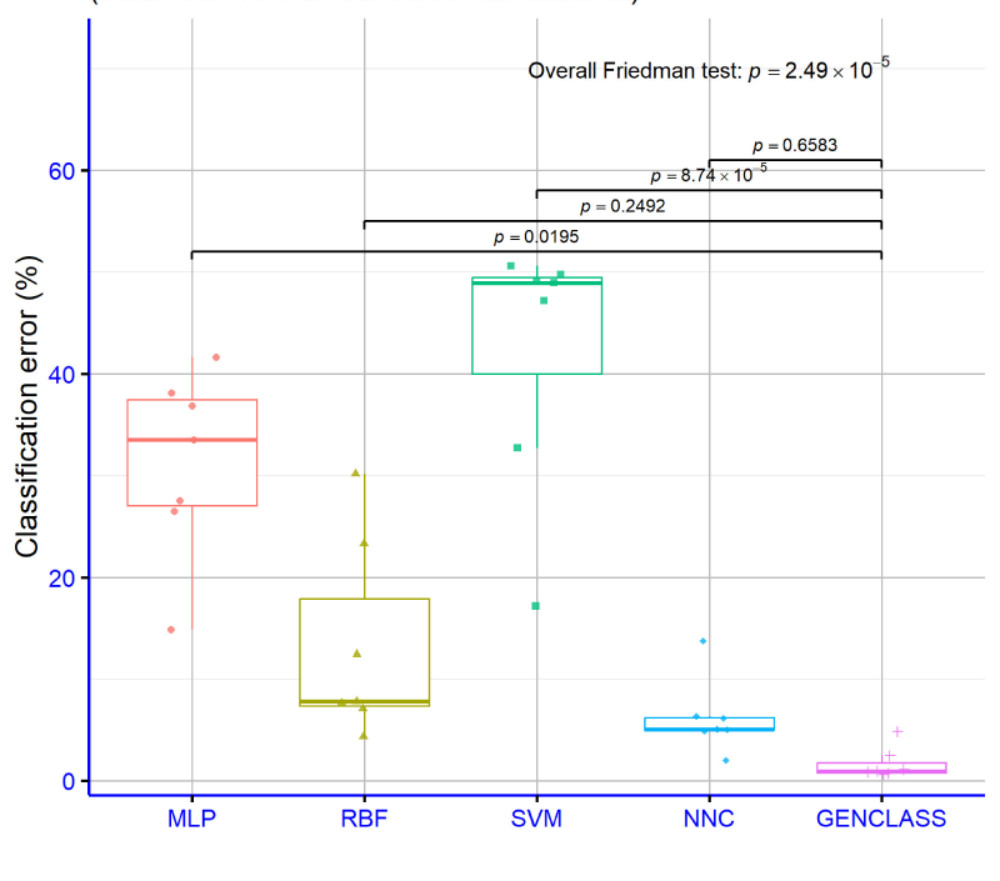
\includegraphics[scale=1.3]{stat-tbl3}


\caption{Statistical Method Comparison (Friedman test with Conover post-hoc) for the results obtained by the application
of various machine learning methods. Common Datasets across all methods \label{fig:Statistical-comparison-for}}
\end{figure}

The dataset related to the CONGO country remains the most challenging
dataset. A possible explanation for this outcome is that, as noted
in the detailed Dataset Description in Section 2.2, the Congo region
does not exhibit balanced class distributions compared to the other
areas. This imbalance likely contributes to the slight deviation observed
relative to the rest of our data.

The \Figref{Precision-and-recall} reports precision and recall
for the three learning models (MLP, RBF, and GENCLASS) across the
seven regions (ARABIA, CAPETOWN, GREECE, ICELAND, CONGO, SVALBARD,
TURKEY).\\
 Precision reflects the purity of positive predictions (the
fraction of predicted positives that are correct), whereas recall
reflects the detection rate of the actual positives (the fraction
of true positives that are correctly identified).\\
 GENCLASS consistently
achieves the best performance on both metrics for all regions, exhibiting
near-ceiling values with limited variation (precision approximately
0.950-0.996 and recall approximately 0.946-0.996).\\
 RBF is generally
the second-best approach and reaches high values in several regions
(e.g., GREECE/ICELAND/ARABIA/TURKEY around 0.92-0.96), but it degrades
sharply in CAPETOWN and CONGO (precision 0.571 and 0.585, recall 0.735
and 0.644), which is visible as pronounced drops in the corresponding
curve.\\
 MLP yields the weakest results overall, with precision approximately
0.576-0.711 and recall approximately 0.711-0.852, indicating substantially
lower correctness of positive predictions and reduced ability to capture
positive instances compared to the other methods.\\
 Overall, the figure
provides clear empirical evidence that GENCLASS delivers the most
robust and consistently strong classification behavior across regions
while maintaining simultaneously high precision and high recall.

\begin{figure}
	\centering
	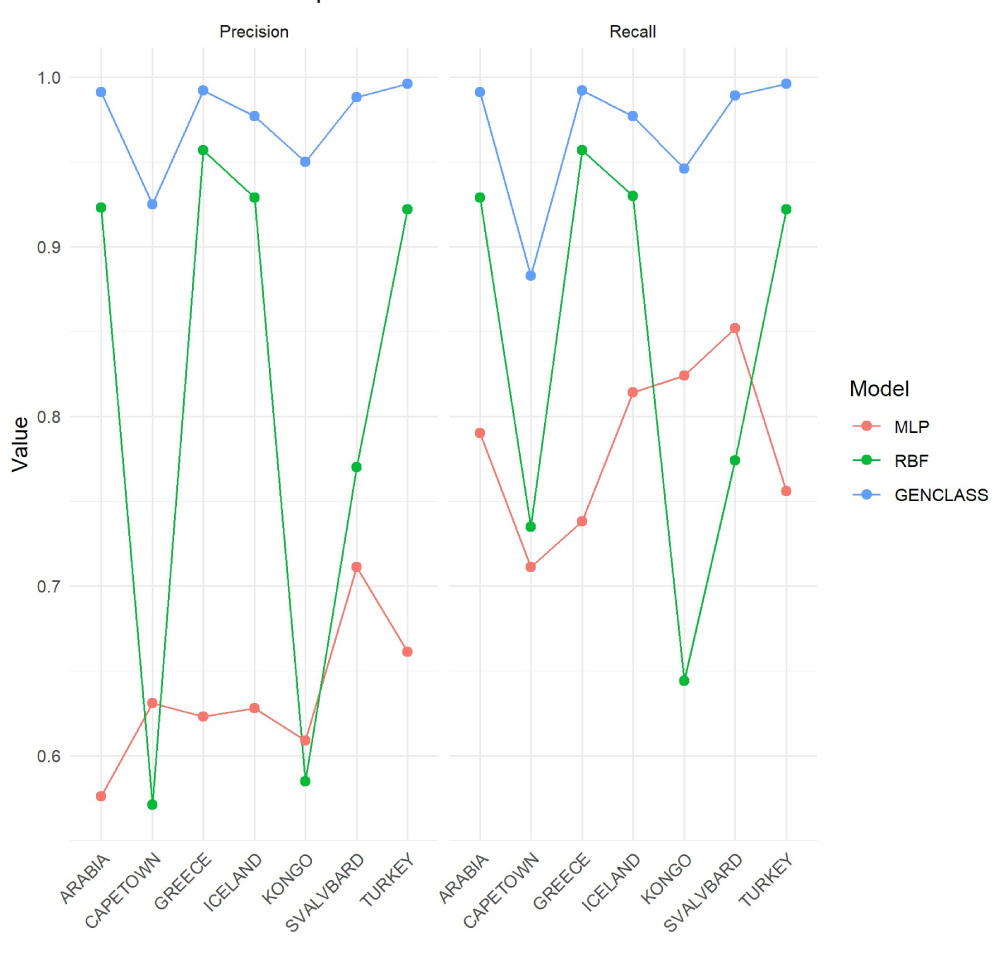
\includegraphics[scale=1.3]{precisionAndRecall} 

\vspace{1em}
\caption{Precision and Recall per model for three methods participated in the conducted
experiments\label{fig:Precision-and-recall}}
\end{figure}


In addition, an indicative diagram showing the learning path for model
GENCLASS and for CONGO dataset is presented in \Figref{An-indicative-plot}.
\begin{figure}[H]
	\centering
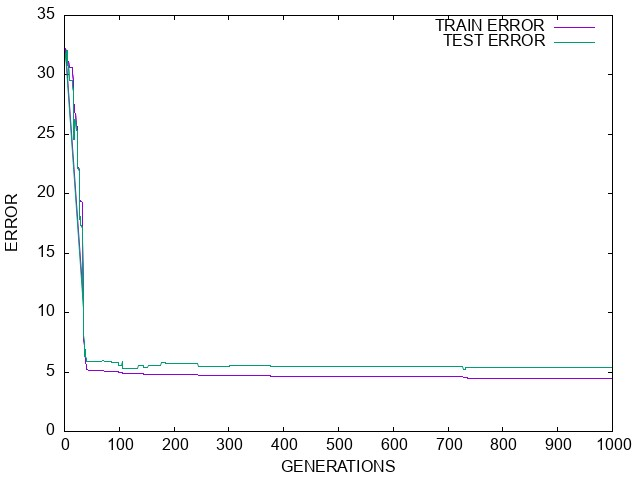
\includegraphics[scale=0.5]{plot_kongo}
\caption{An indicative plot for the method GENCLASS and the dataset CONGO\label{fig:An-indicative-plot}}
\end{figure}
\vspace{-0.1em} 
\clearpage
Moreover, Indicative plots for ROC and PR performance curves are outlined
in \Figref{Indicative-plots-for-ROC} and \Figref{Indicative-plots-for-PR}
respectively.

\begin{figure}[H]
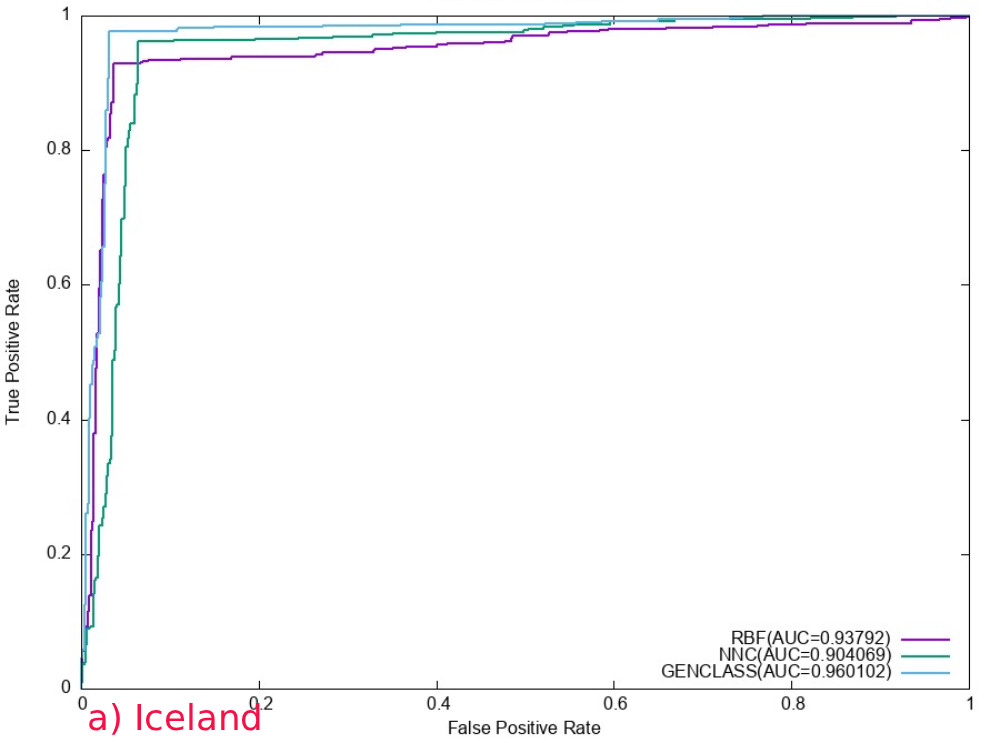
\includegraphics[scale=1]{iceland_roc}
 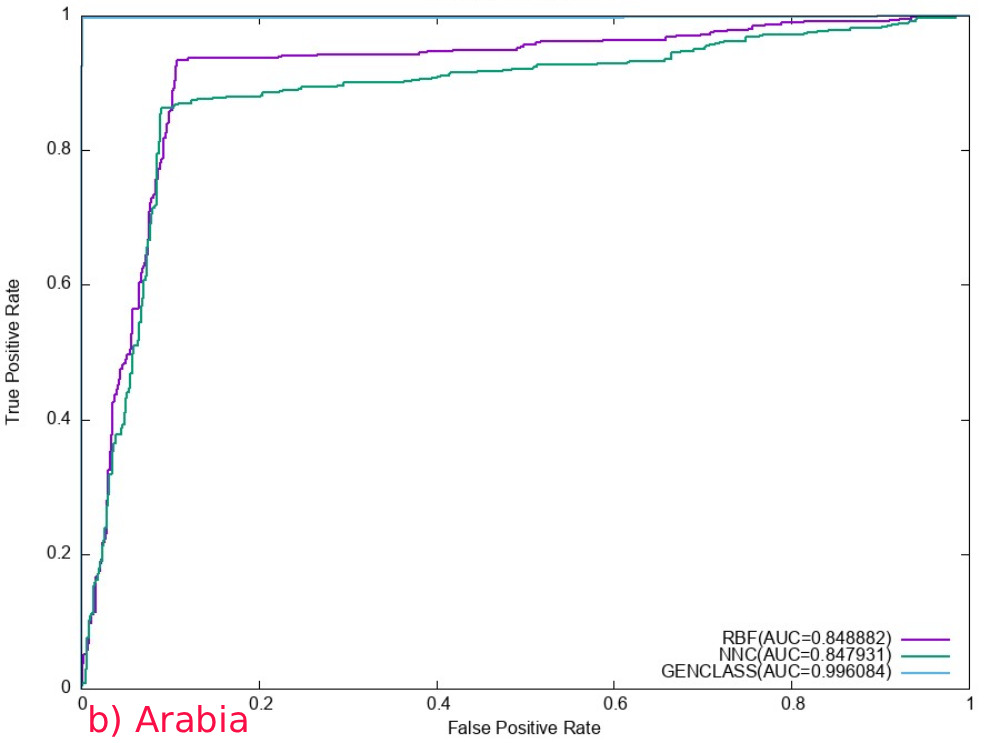
\includegraphics[scale=1]{arabia_roc}
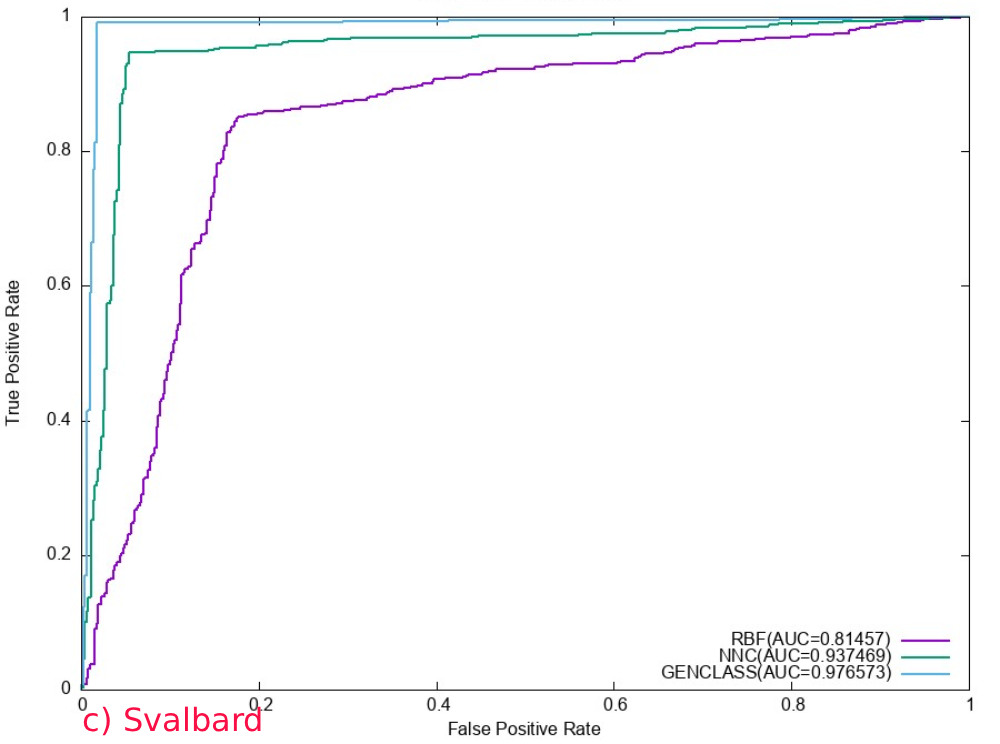
\includegraphics[scale=1]{svalbard_roc}
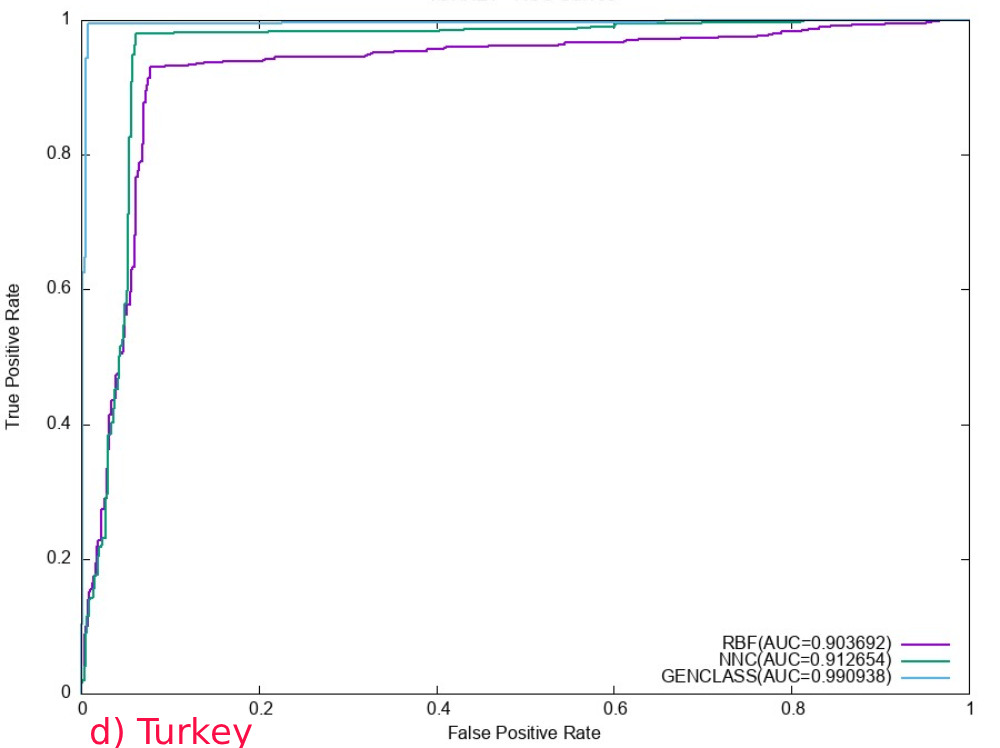
\includegraphics[scale=1]{turkey_roc}

\caption{Indicative plots for the ROC curves, involving the RBF network, the
NNC method and the GENCLASS method\label{fig:Indicative-plots-for-ROC}}
\end{figure}

\begin{figure}[H]
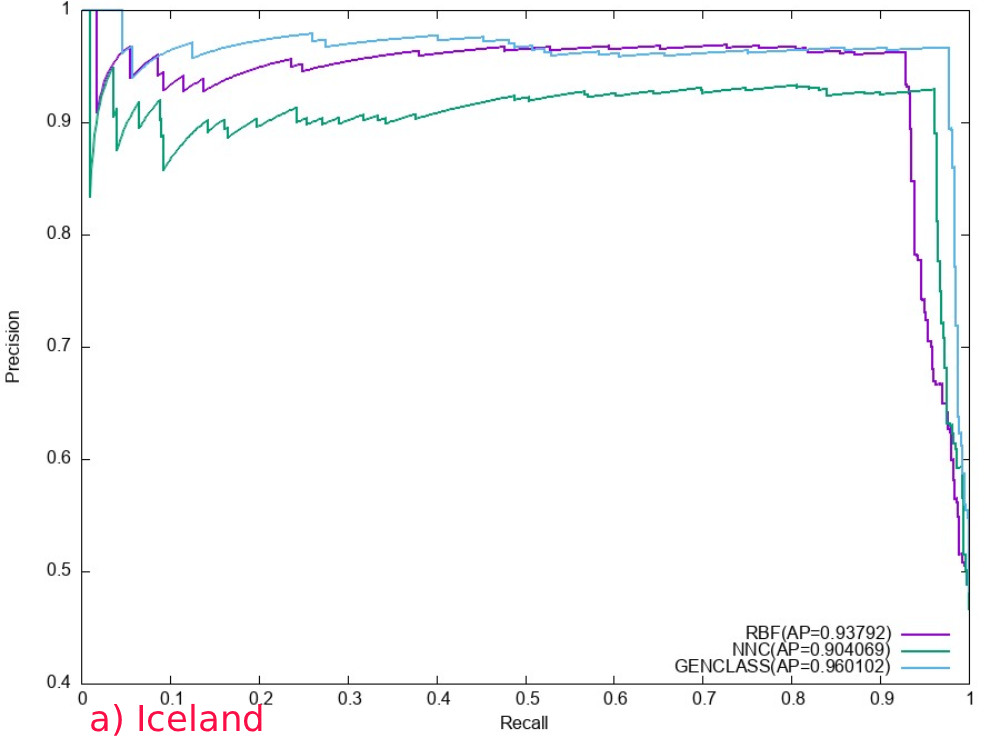
\includegraphics[scale=1]{iceland_pr}
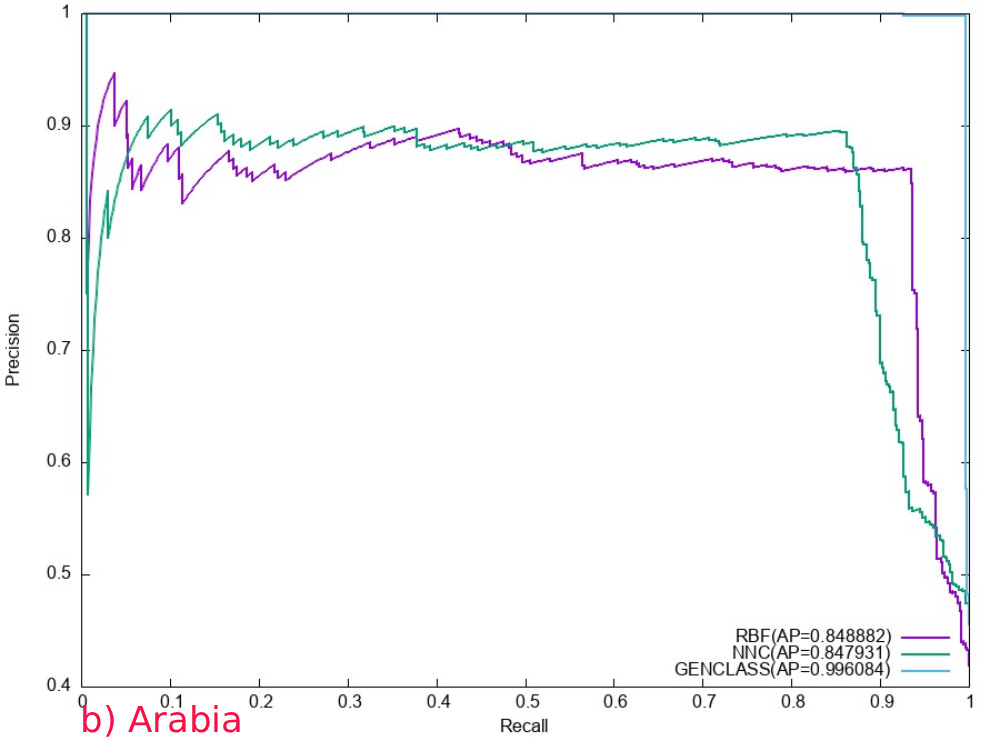
\includegraphics[scale=1]{arabia_pr}
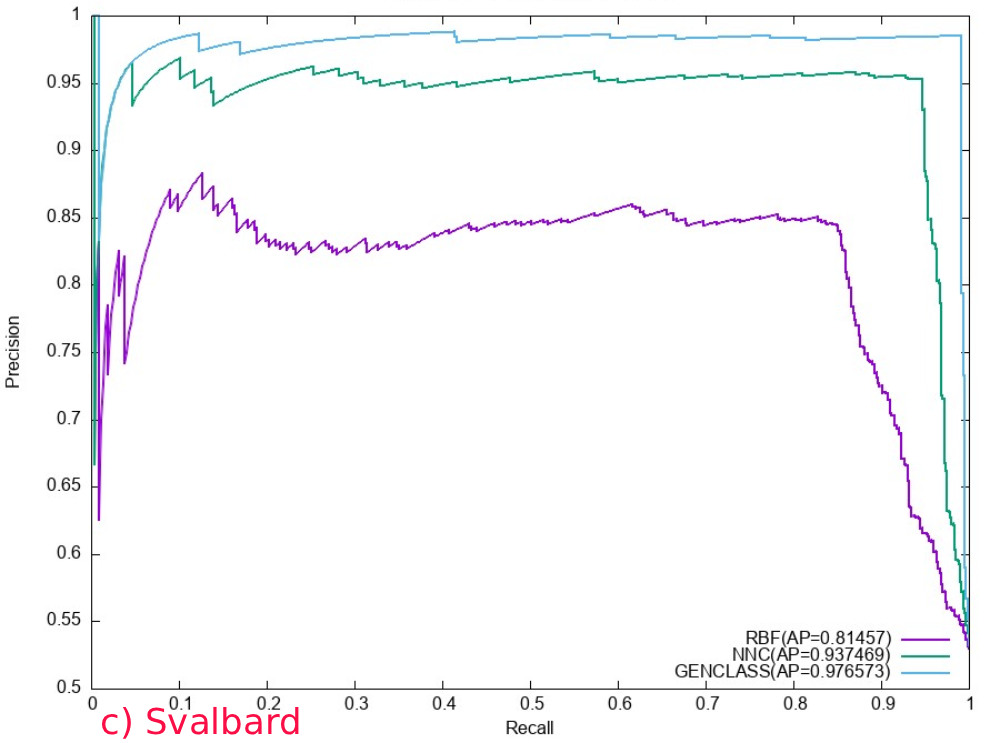
\includegraphics[scale=1]{svalbard_pr}
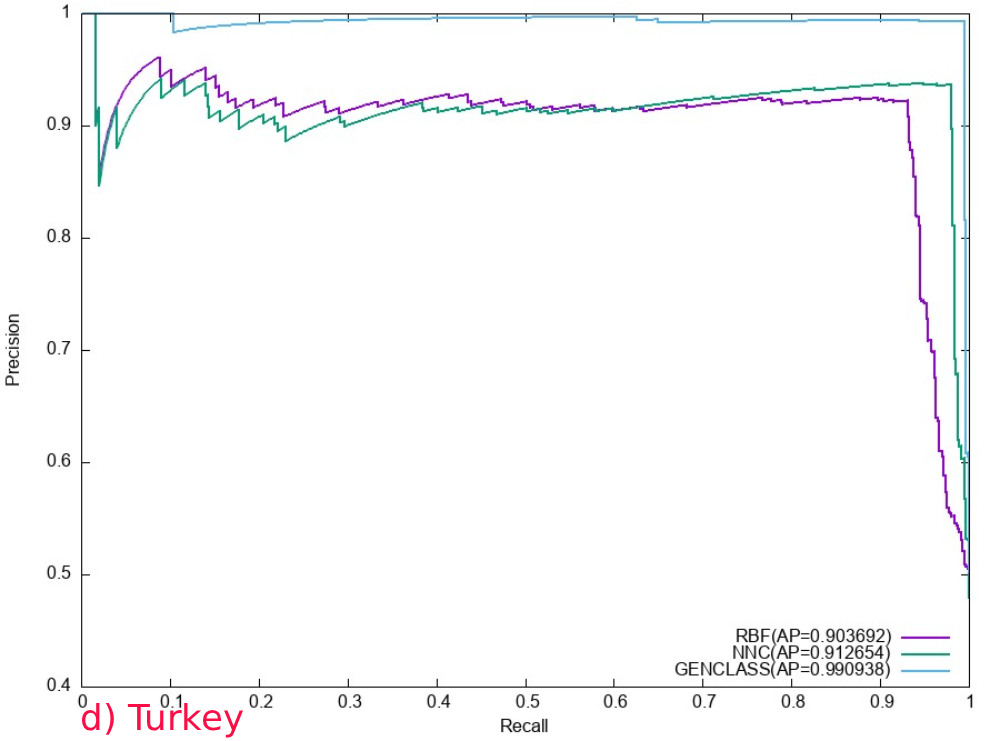
\includegraphics[scale=1]{turkey_pr}

\caption{Indicative plots for the PR curves for the RBF network, the NNC method
and the GENCLASS method\label{fig:Indicative-plots-for-PR}}
\end{figure}

As an example of rule production from the GENCLASS method, consider
the program presented in Algorithm \ref{alg:An-example-of} for the
Greece dataset. As can be observed, the rule-generation method produces
rules in a form that is understandable by humans (the above program
can also be exported to actual C++ and Python code through the available
software). Furthermore, for the effective creation of a classification
program, it is not necessary to use all the features of the dataset
under study.\textquotedblright{}


\begin{algorithm}[H]
	\caption{An example of classification program for the Greece dataset}
	\label{alg:An-example-of}
	\begin{algorithmic}[1]
		
		\If{$x_{26} \ge \frac{-61.4 + x_{3}}{-1.085}$ 
			\textbf{ and } $x_{11} \le x_{4}$ 
			\textbf{ and } $\neg(x_{1} < -58.007 
			\textbf{ or } 
			x_{21} > (-561.6) \cdot (-563.231) \cdot (x_{28} + x_{1} - 77.456)
			)$
			\textbf{ and } $x_{12} \ge x_{5} - 47.804$
		}
		\State CLASS = 0
		\Else
		\State CLASS = 1
		\EndIf
		
	\end{algorithmic}
\end{algorithm}




\clearpage

\subsection{\textmd{Experiments with the number of chromosomes}}

In \Tabref{Table-7-Experimental-results-on-1} evaluates the sensitivity
of the proposed model to the number of chromosomes $N_{c}$, using
classification error percentages as the performance metric (lower
is better).\\ A clear and nearly monotonic improvement is observed as
$N_{c}$ increases from 50 to 1000: the mean error (AVERAGE row) drops
from 3.21\% to 1.46\%, i.e., an absolute reduction of 1.75 percentage
points corresponding to an approximate 54.5\% relative decrease. Most
of the gain is realized up to $N_{c}$=500 (3.21\%\textrightarrow 2.68\%\textrightarrow 2.17\%\textrightarrow 1.66\%),
whereas the additional improvement from 500 to 1000 is smaller (1.66\%\textrightarrow 1.46\%,
a 0.20 decrease), indicating diminishing returns for very large chromosome
counts. At the dataset level, the largest relative reductions from
$N_{c}$=50 to $N_{c}$=1000 occur for ARABIA (2.52\%\textrightarrow 0.54\%, the improvement amounted
\textasciitilde 78.6\%) and for TURKEY (2.37\%\textrightarrow 0.57\%,the improvement amounted
\textasciitilde 75.9\%).\\ In contrast, ICELAND exhibits a smaller
but consistent overall reduction (3.22\%\textrightarrow 2.14\%, to \textasciitilde 33.5\%)
and a slight non-monotonic fluctuation at $N_{c}$=100 (3.27\% vs.
3.22\%), which is corrected for higher$N_{c}$. CONGO remains the
most challenging dataset across all settings (8.86\% at $N_{c}$=50
and 4.39\% at $N_{c}$=1000), implying that increasing $N_{c}$ substantially
improves performance but does not fully remove the intrinsic difficulty
associated with that region\textquoteright s data structure. \\ Importantly,
cross-dataset variability also decreases with $N_{c}$: the maximum
error decreases from 8.86\% to 4.39\% and the range (max-min) shrinks
from 7.08 to 3.85 percentage points, while the standard deviation
of errors across datasets declines from about 2.54 to 1.40, suggesting
more uniform generalization when using larger chromosome counts.

\begin{table}[H]
	\centering
\begin{tabular}{|c|c|c|c|c|c|}
\hline
\textbf{Dataset} & \textbf{$N_{c}=50$} & \textbf{$N_{c}=100$} & \textbf{$N_{c}=200$} & \textbf{$N_{c}=500$} & \textbf{$N_{c}=1000$}\tabularnewline
\hline
\hline
\textbf{Cape Town} & 1.85\% & 1.63\% & 1.40\% & 0.97\% & 0.78\%\tabularnewline
\hline
\textbf{Greece} & 1.78\% & 1.24\% & 1.13\% & 0.85\% & 0.83\%\tabularnewline
\hline
\textbf{Iceland} & 3.22\% & 3.27\% & 2.75\% & 2.47\% & 2.14\%\tabularnewline
\hline
\textbf{Congo} & 8.86\% & 8.18\% & 6.31\% & 4.84\% & 4.39\%\tabularnewline
\hline
\textbf{Arabia} & 2.52\% & 1.32\% & 1.26\% & 0.73\% & 0.54\%\tabularnewline
\hline
\textbf{Svalbard} & 1.89\% & 1.58\% & 1.30\% & 1.11\% & 0.94\%\tabularnewline
\hline
\textbf{Turkey} & 2.37\% & 1.57\% & 1.06\% & 0.63\% & 0.57\%\tabularnewline
\hline
\textbf{Average} & \textbf{3.21\%} & \textbf{2.68\%} & \textbf{2.17\%} & \textbf{1.66\%} & \textbf{1.46\%}\tabularnewline
\hline
\end{tabular}
\vspace{1em}
\caption{Experimental results on the provided datasets using the proposed method
and a series of values for the number of chromosomes $N_{c}$.\label{tab:Table-7-Experimental-results-on-1}}
\end{table}

\clearpage
In \Figref{stat-tb17.png} clearly illustrates that increasing the
number of chromosomes leads to lower classification error across essentially
all datasets, with the mean performance (AVERAGE, black dashed line)
following a steady downward trend. The improvement is most pronounced
from small $N_{c}$ values up to approximately$N_{c}$=500, after
which the error continues to decrease but at a slower rate, indicating
diminishing returns for very large chromosome counts. Moreover, the
dataset-specific curves become slightly more clustered as $N_{c}$
increases, suggesting a more uniform behavior of the proposed model
across regions.

Increasing the number of chromosomes will allow the genetic algorithm
underlying the GENCLASS technique to perform a more thorough exploration
of the problem\textquoteright s search space and to generate a larger
number of classification rules. In this way, higher accuracy on the
model\textquoteright s error in the test set can be achieved. Naturally,
this will also lead to increased training times; however, this drawback
can be mitigated through the use of parallel Genetic Algorithms.

\begin{figure}[H]
	\centering
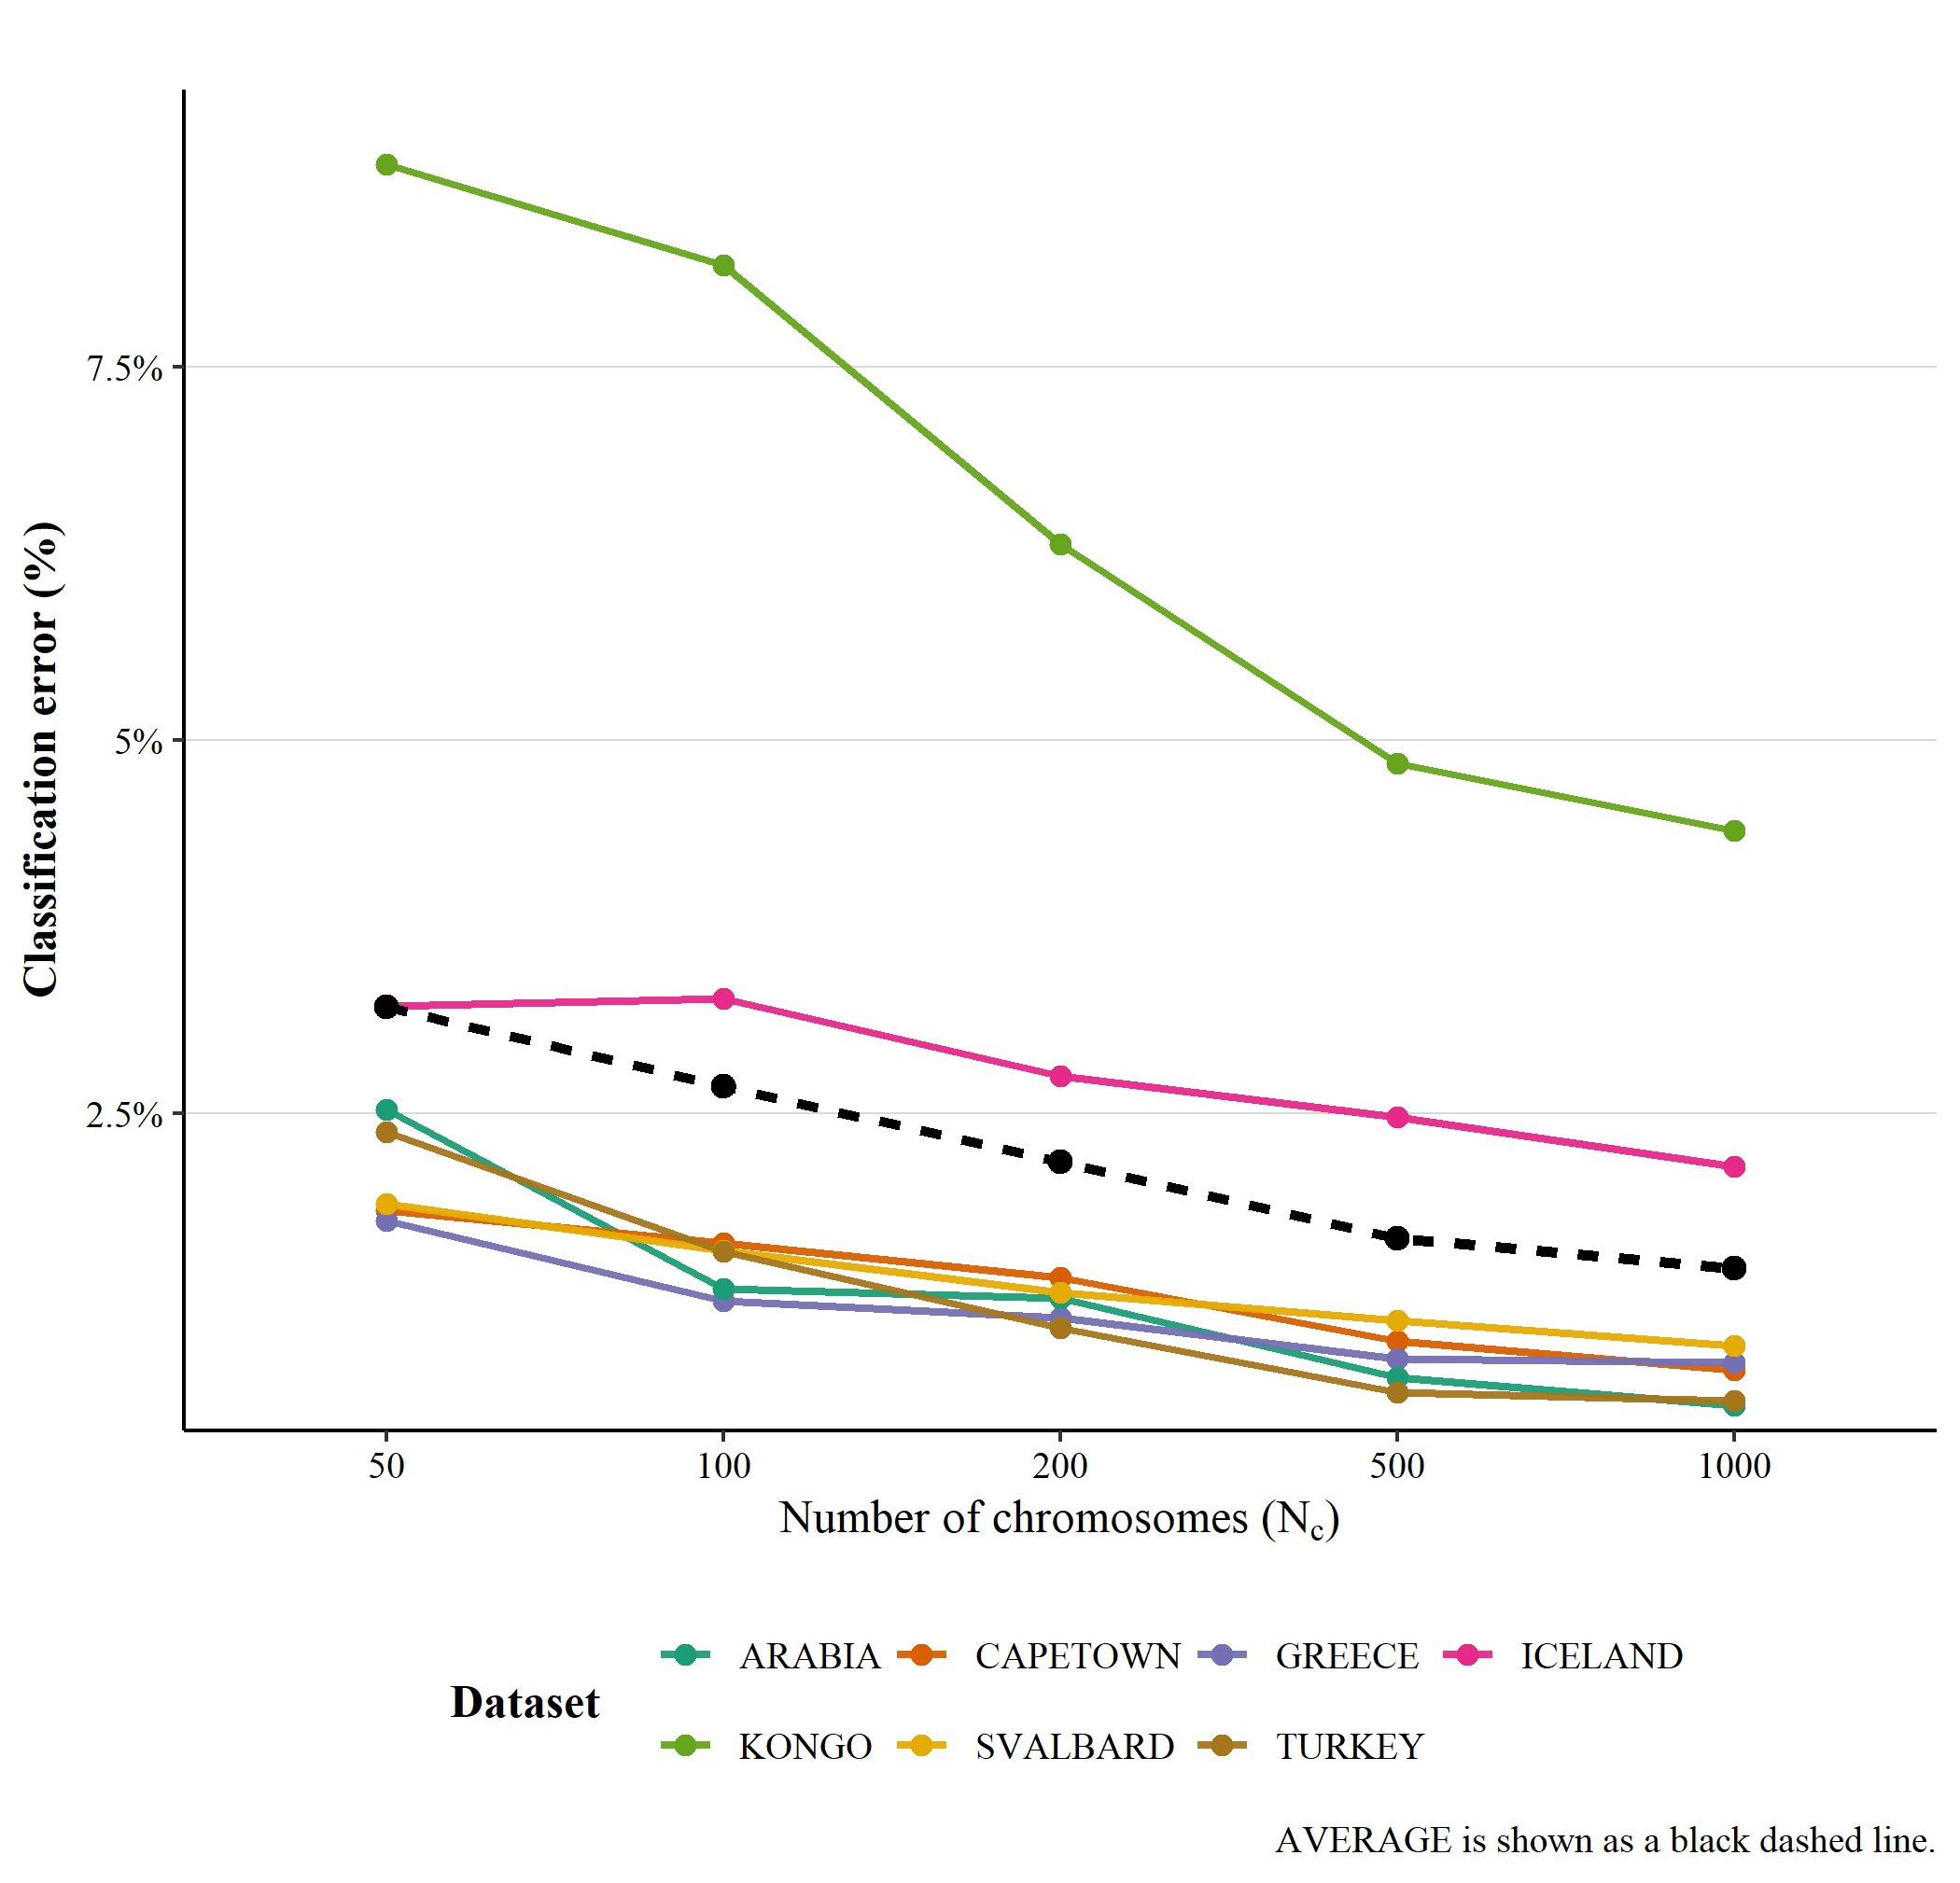
\includegraphics[scale=0.8]{stat_tbl7}

\caption{This figure shows the effect of changing the number of Chromosomes $N_{c}$
on the learning Classification Error of the proposed technique for a series of datasets (Table 7)\label{fig:stat-tb17.png}}
\end{figure}


\clearpage
Also, the average execution time for the proposed method and a variety
of values for the $N_{c}$ parameter is outlined in \Figref{Average-execution-time}.\\
As it was expected, the execution time increases rapidly as the number
of chromosomes increases.

\begin{figure}[H]
	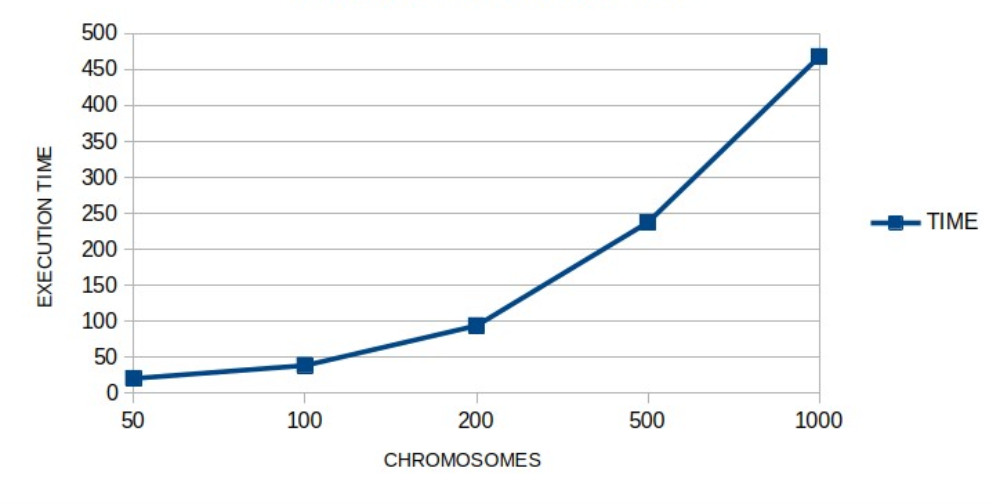
\includegraphics[scale=1.7]{exectime}

\caption{Average Execution time for the proposed method and different values
of parameter $N_{c}$\label{fig:Average-execution-time}}
\end{figure}

\clearpage
\subsection{\textmd{Experiments with the number of generations\label{subsec:Experiments-with-the}}}

Table \ref{tab:Table-8-Experimental-results-on-Ng} investigates the effect
of the number of generations $N_{g}$ on the proposed model, using
classification error percentages as the evaluation metric (lower is
better). The overall trend is strongly improving with increasing$N_{g}$:
the mean error (AVERAGE) decreases from 4.46\% at $N_{g}$=50 to 1.45\%
at $N_{g}$=2000, corresponding to a 3.01 percentage-point reduction
and an approximate 67.4\% relative decrease.\\
 The gains are not evenly
distributed across increments: 50\textrightarrow 100 (-0.99), 100\textrightarrow 200
(-0.82), 200\textrightarrow 1000 (-0.98), and 1000\textrightarrow 2000
(-0.21), indicating diminishing returns beyond 1000 generations, where
additional computational effort yields smaller improvements in the
mean error. At the dataset level, all regions improve substantially
from $N_{g}$=50 to $N_{g}$=2000, with the largest relative reductions
observed for TURKEY (2.63\%\textrightarrow 0.37\%,the improvement amounted \textasciitilde 85.9\%)
and ARABIA (3.03\%\textrightarrow 0.63\%, the improvement amounted \textasciitilde 79.2\%).\\
CONGO also improves markedly (14.12\%\textrightarrow 4.18\%,the improvement amounted \textasciitilde 70.4\%)
but remains the most challenging dataset across all settings, consistently
exhibiting the highest errors. ICELAND shows the smallest overall
relative improvement (4.32\%\textrightarrow 2.58\%, with \textasciitilde 40.3\%)
and a slight degradation from $N_{g}$=1000 to$N_{g}$ =2000 (2.47\%\textrightarrow 2.58\%),
suggesting that for certain datasets additional generations may introduce
over-training effects and/or stochastic variability that partially
offsets expected gains. The slight degradation in the ICELAND dataset
between$N_{g}$ =1000 and $N_{g}$=2000 can be attributed to stochastic
fluctuations in the evolutionary search and dataset\nobreakdash-specific
characteristics that limit further improvement beyond a certain number
of generations.\\
 Increasing $N_{g}$ also reduces cross-dataset variability:
the maximum error drops from 14.12\% to 4.18\% and the range (max--min)
shrinks from 11.92 to 3.81 percentage points, while the standard deviation
across datasets decreases from about 4.00 to 1.30, supporting a more
uniform generalization profile at higher$N_{g}$.

\begin{table}[H]
	\centering
\begin{tabular}{|c|c|c|c|c|c|}
\hline
\textbf{Dataset} & $N_{g}=50$ & $N_{g}=100$ & $N_{g}=200$ & $N_{g}=1000$ & $N_{g}=2000$\tabularnewline
\hline
\hline
\textbf{Cape Town} & 2.40\% & 1.96\% & 1.60\% & 0.97\% & 0.73\%\tabularnewline
\hline
\textbf{Greece} & 2.20\% & 1.74\% & 1.32\% & 0.85\% & 0.82\%\tabularnewline
\hline
\textbf{Iceland} & 4.32\% & 3.75\% & 3.05\% & 2.47\% & 2.58\%\tabularnewline
\hline
\textbf{Congo} & 14.12\% & 10.49\% & 7.91\% & 4.84\% & 4.18\%\tabularnewline
\hline
\textbf{Arabia} & 3.03\% & 2.35\% & 1.67\% & 0.73\% & 0.63\%\tabularnewline
\hline
\textbf{Svalbard} & 2.50\% & 1.98\% & 1.54\% & 1.11\% & 0.85\%\tabularnewline
\hline
\textbf{Turkey} & 2.63\% & 1.97\% & 1.38\% & 0.63\% & 0.37\%\tabularnewline
\hline
\textbf{Average} & \textbf{4.46\%} & \textbf{3.46\%} & \textbf{2.64\%} & \textbf{1.66\%} & \textbf{1.45\%}\tabularnewline
\hline
\end{tabular}
\vspace{1em}
\caption{Experimental results on the provided datasets using the proposed method
and a series of values for the number of generations $N_{g}$.\label{tab:Table-8-Experimental-results-on-Ng}}
\end{table}


\clearpage
In \Figref{The-impact-of-stat-tb18} shows that increasing the number
of generations also yields a systematic reduction in classification
error, with the mean curve (AVERAGE) improving markedly when moving
from few to many generations. The largest gains are achieved up to
roughly $N_{g}$=1000, while the transition from$N_{g}$=1000 to $N_{g}$
=2000 exhibits a clear flattening of the curves, implying that additional
computational effort produces smaller marginal improvements. Although
minor dataset-specific fluctuations may occur at the final step, the
overall pattern confirms that larger$N_{g}$ enhances generalization
and reduces error.

\begin{figure}[H]
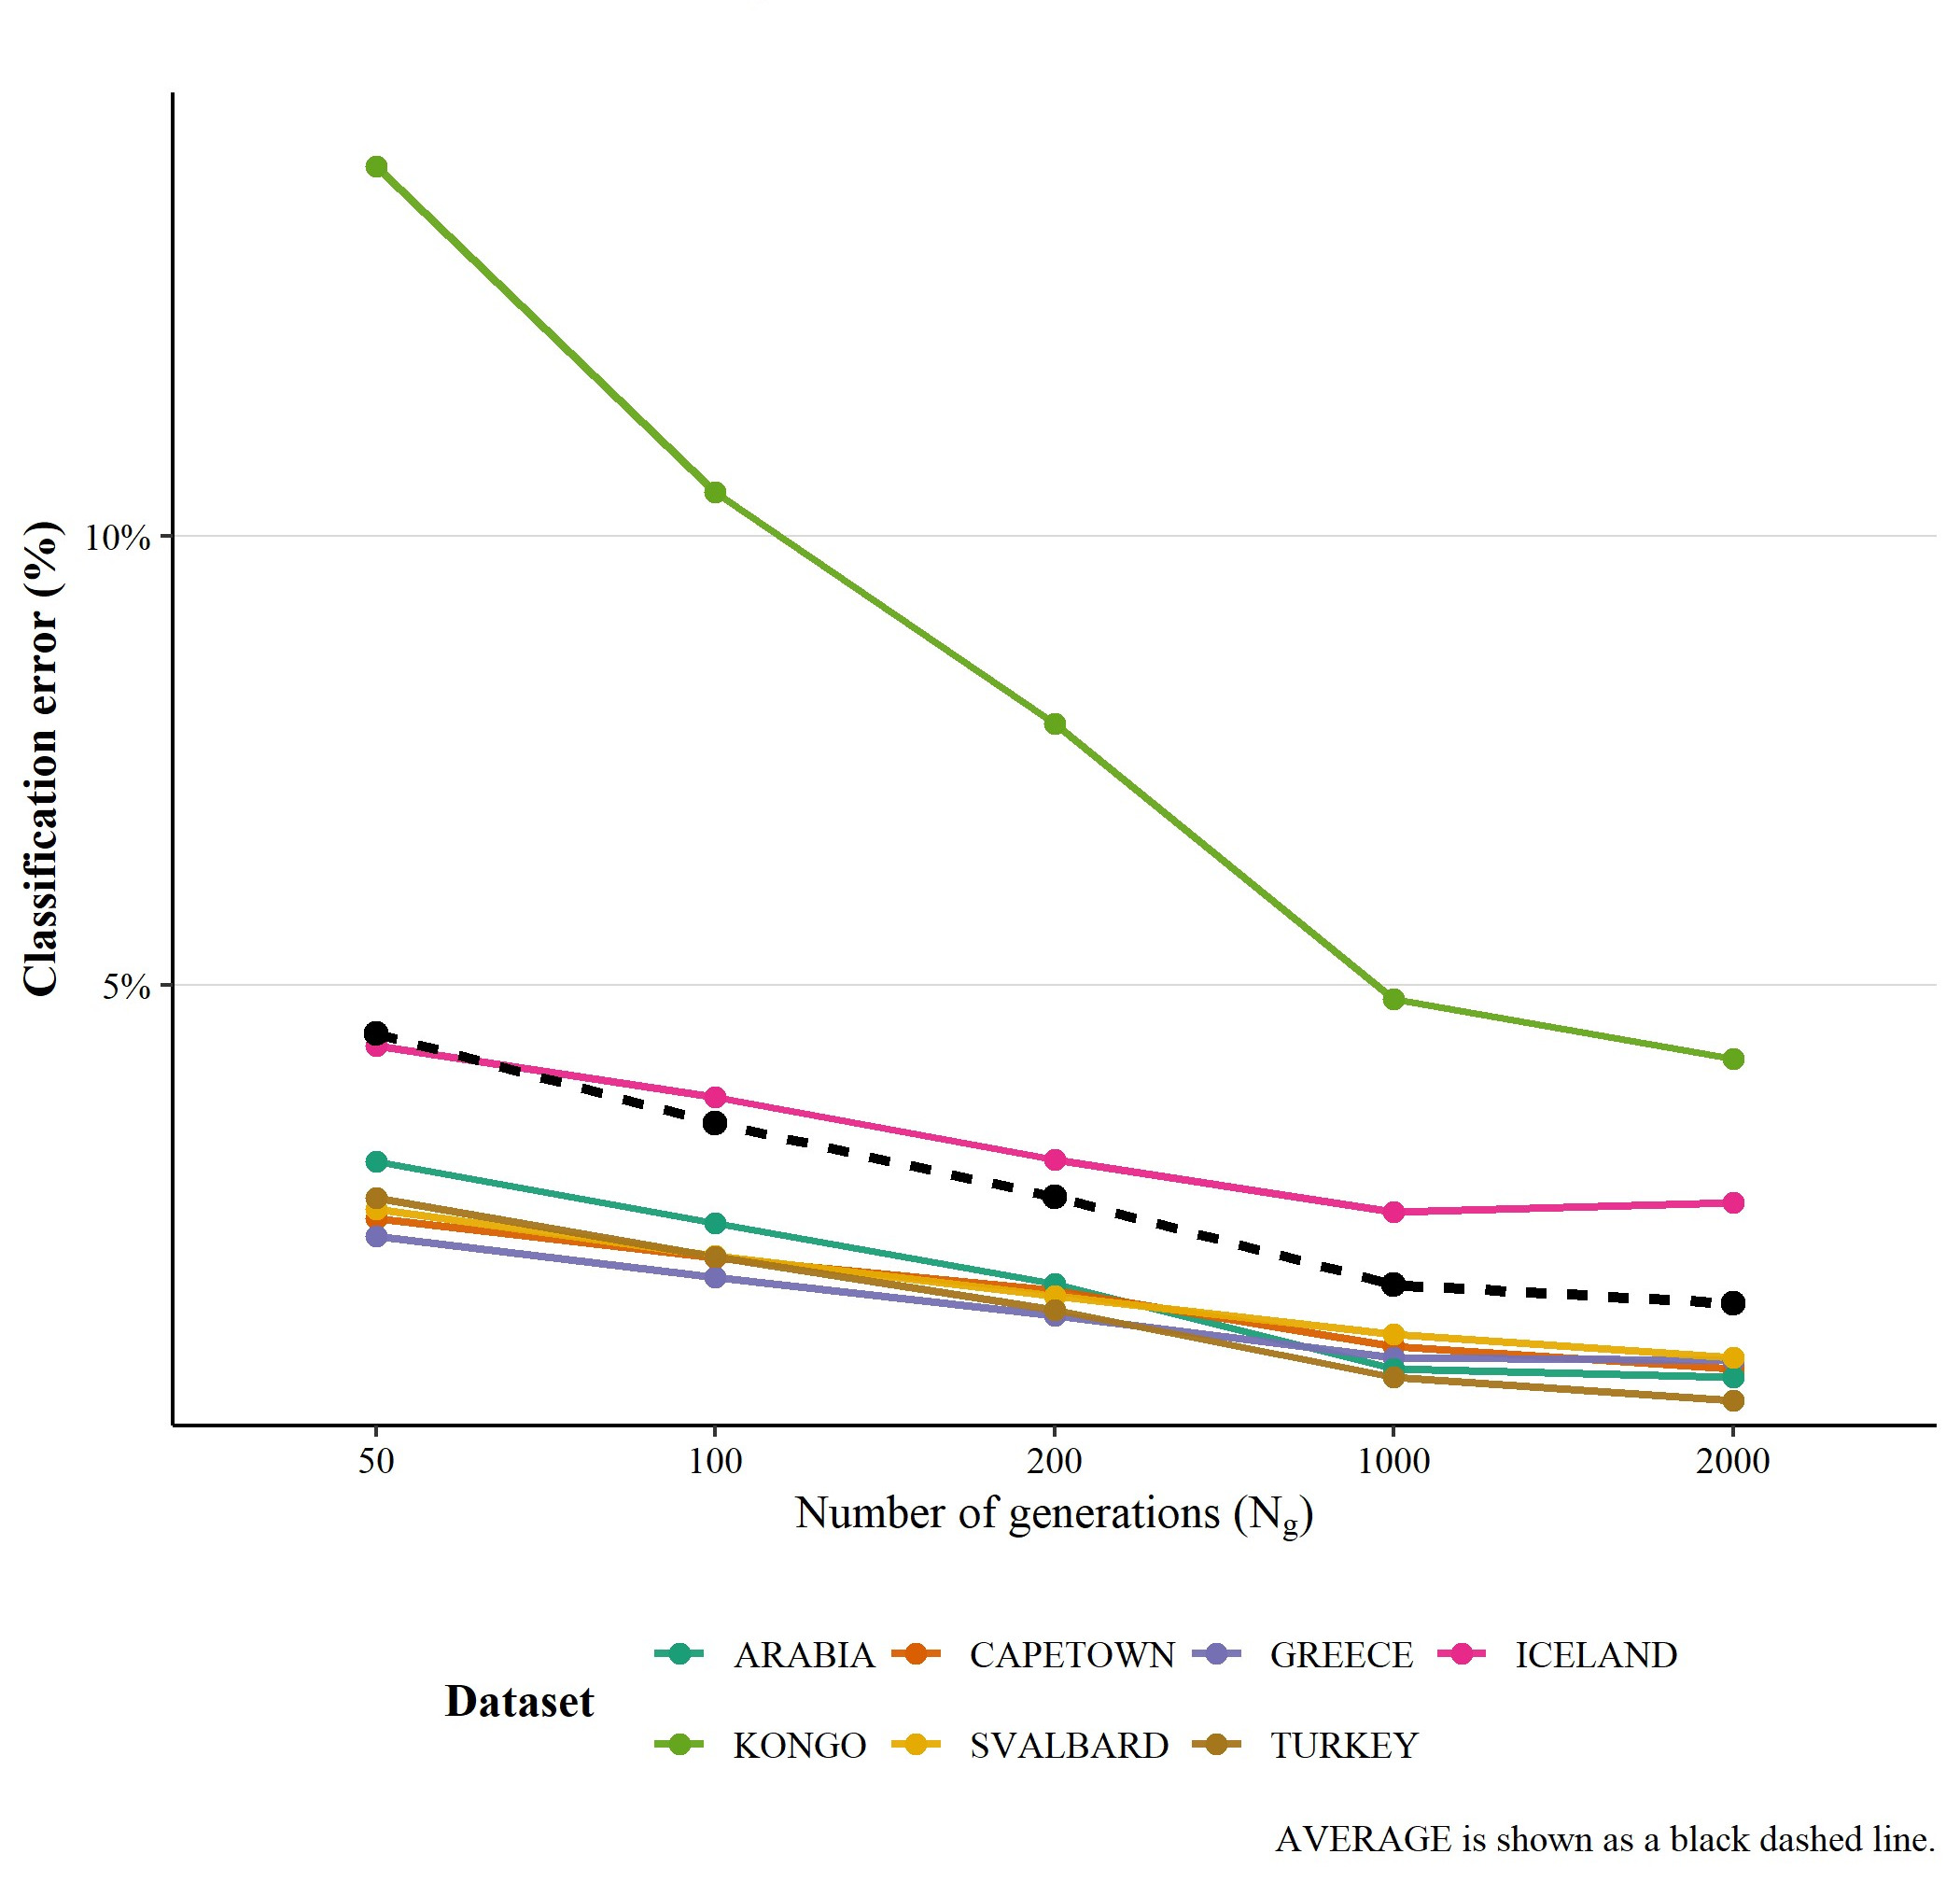
\includegraphics[scale=0.8]{stat_tbl8}

\caption{The impact of altering the number of Generations $N_{g}$ to the Classification
Error of the proposed method (Table 8)\label{fig:The-impact-of-stat-tb18}}
\end{figure}

As shown here and according to established GA theory, increasing the
number of generations allows the evolutionary process to explore a
larger portion of the search space and refine candidate solutions
over time, leading to more stable convergence and improved generalization
across datasets.


\clearpage
\subsection{\textmd{Experiments with the RBF network}}

Another experiment was conducted where the RBF network was used as
the classification model and the number of weights $H$ was varied
from 10 to 30 and the corresponding results are listed in \Tabref{Table-9-Experimental-RBF-results-using}

\begin{table}[H]
	\centering
\begin{tabular}{|c|c|c|c|c|c|c|}
\hline
\textbf{Dataset} &
\centering
$H=10$
 &
\centering
$H=15$
 &
\centering
$H=20$
 &
\centering
$H=25$
 &
\centering
RBF
$H=30$
 & GENCLASS\tabularnewline
\hline
\hline
\textbf{Cape Town} & 12.43\% & 11.50\% & 10.77\% & 10.55\% & 10.41\% & 0.97\%\tabularnewline
\hline
\textbf{Greece} & 4.34\% & 3.34\% & 2.98\% & 9.06\% & 18.69\% & 0.85\%\tabularnewline
\hline
\textbf{Iceland} & 7.09\% & 4.79\% & 4.06\% & 3.33\% & 3.13\% & 2.47\%\tabularnewline
\hline
\textbf{Congo} & 30.16\% & 17.59\% & 19.93\% & 21.69\% & 21.21\% & 4.84\%\tabularnewline
\hline
\textbf{Arabia} & 7.62\% & 4.35\% & 3.40\% & 2.96\% & 2.81\% & 0.73\%\tabularnewline
\hline
\textbf{Svalbard} & 23.30\% & 9.65\% & 7.74\% & 6.92\% & 6.44\% & 1.11\%\tabularnewline
\hline
\textbf{Turkey} & 7.81\% & 7.00\% & 7.54\% & 6.77\% & 7.87\% & 0.63\%\tabularnewline
\hline
\textbf{Average} & \textbf{13.25\%} & \textbf{8.32\%} & \textbf{8.06\%} & \textbf{8.75\%} & \textbf{10.08\%} & \textbf{1.66\%}\tabularnewline
\hline
\end{tabular}
\vspace{1em}
\caption{Experimental results using different number for the weights $H$ of
the RBF network.\label{tab:Table-9-Experimental-RBF-results-using}}
\end{table}


The last  \Figref{RBF-Sensitivity-to} is a heatmap of classification error
(Error \%) for the RBF model under different numbers of hidden nodes
H, together with a GENCLASS reference column. Each row corresponds
to one region/dataset (CAPETOWN, GREECE, ICELAND, CONGO, ARABIA, SVALBARD,
TURKEY), while the last row (AVERAGE) reports the mean error across
all regions.\\
 Each column represents a different RBF configuration
($H=10$, 15, 20, 25, 30), and the final column reports GENCLASS.
The numerical error percentages are printed inside each cell, and
the color intensity encodes the magnitude of the error (darker color
indicates lower error).\\
 The heatmap shows that increasing H often
improves RBF performance initially, but the trend is not monotonic
and degradation is observed for larger H in some regions, which is
consistent with overfitting; for example, in GREECE the error remains
low up to $H=20$ but increases sharply at $H=25$ and $H=30$, while
in CONGO the best performance occurs at a smaller H and then worsens
as H grows.\\
 In the AVERAGE row, the best mean RBF performance occurs
around $H=20$, whereas larger settings ($H=25,H=30$) lead to higher
mean error, highlighting a saturation regime and diminishing returns.\\
Across all regions, GENCLASS achieves markedly lower error than any
tested RBF setting, indicating a consistently stronger reference performance
against which RBF sensitivity to hidden-layer size can be assessed.
All values in the figure are taken directly from the raw Excel table
(without formatting) and visually summarize both the initial gains
from increasing H and the potential performance drop when H becomes
excessively large.

\begin{figure}[H]
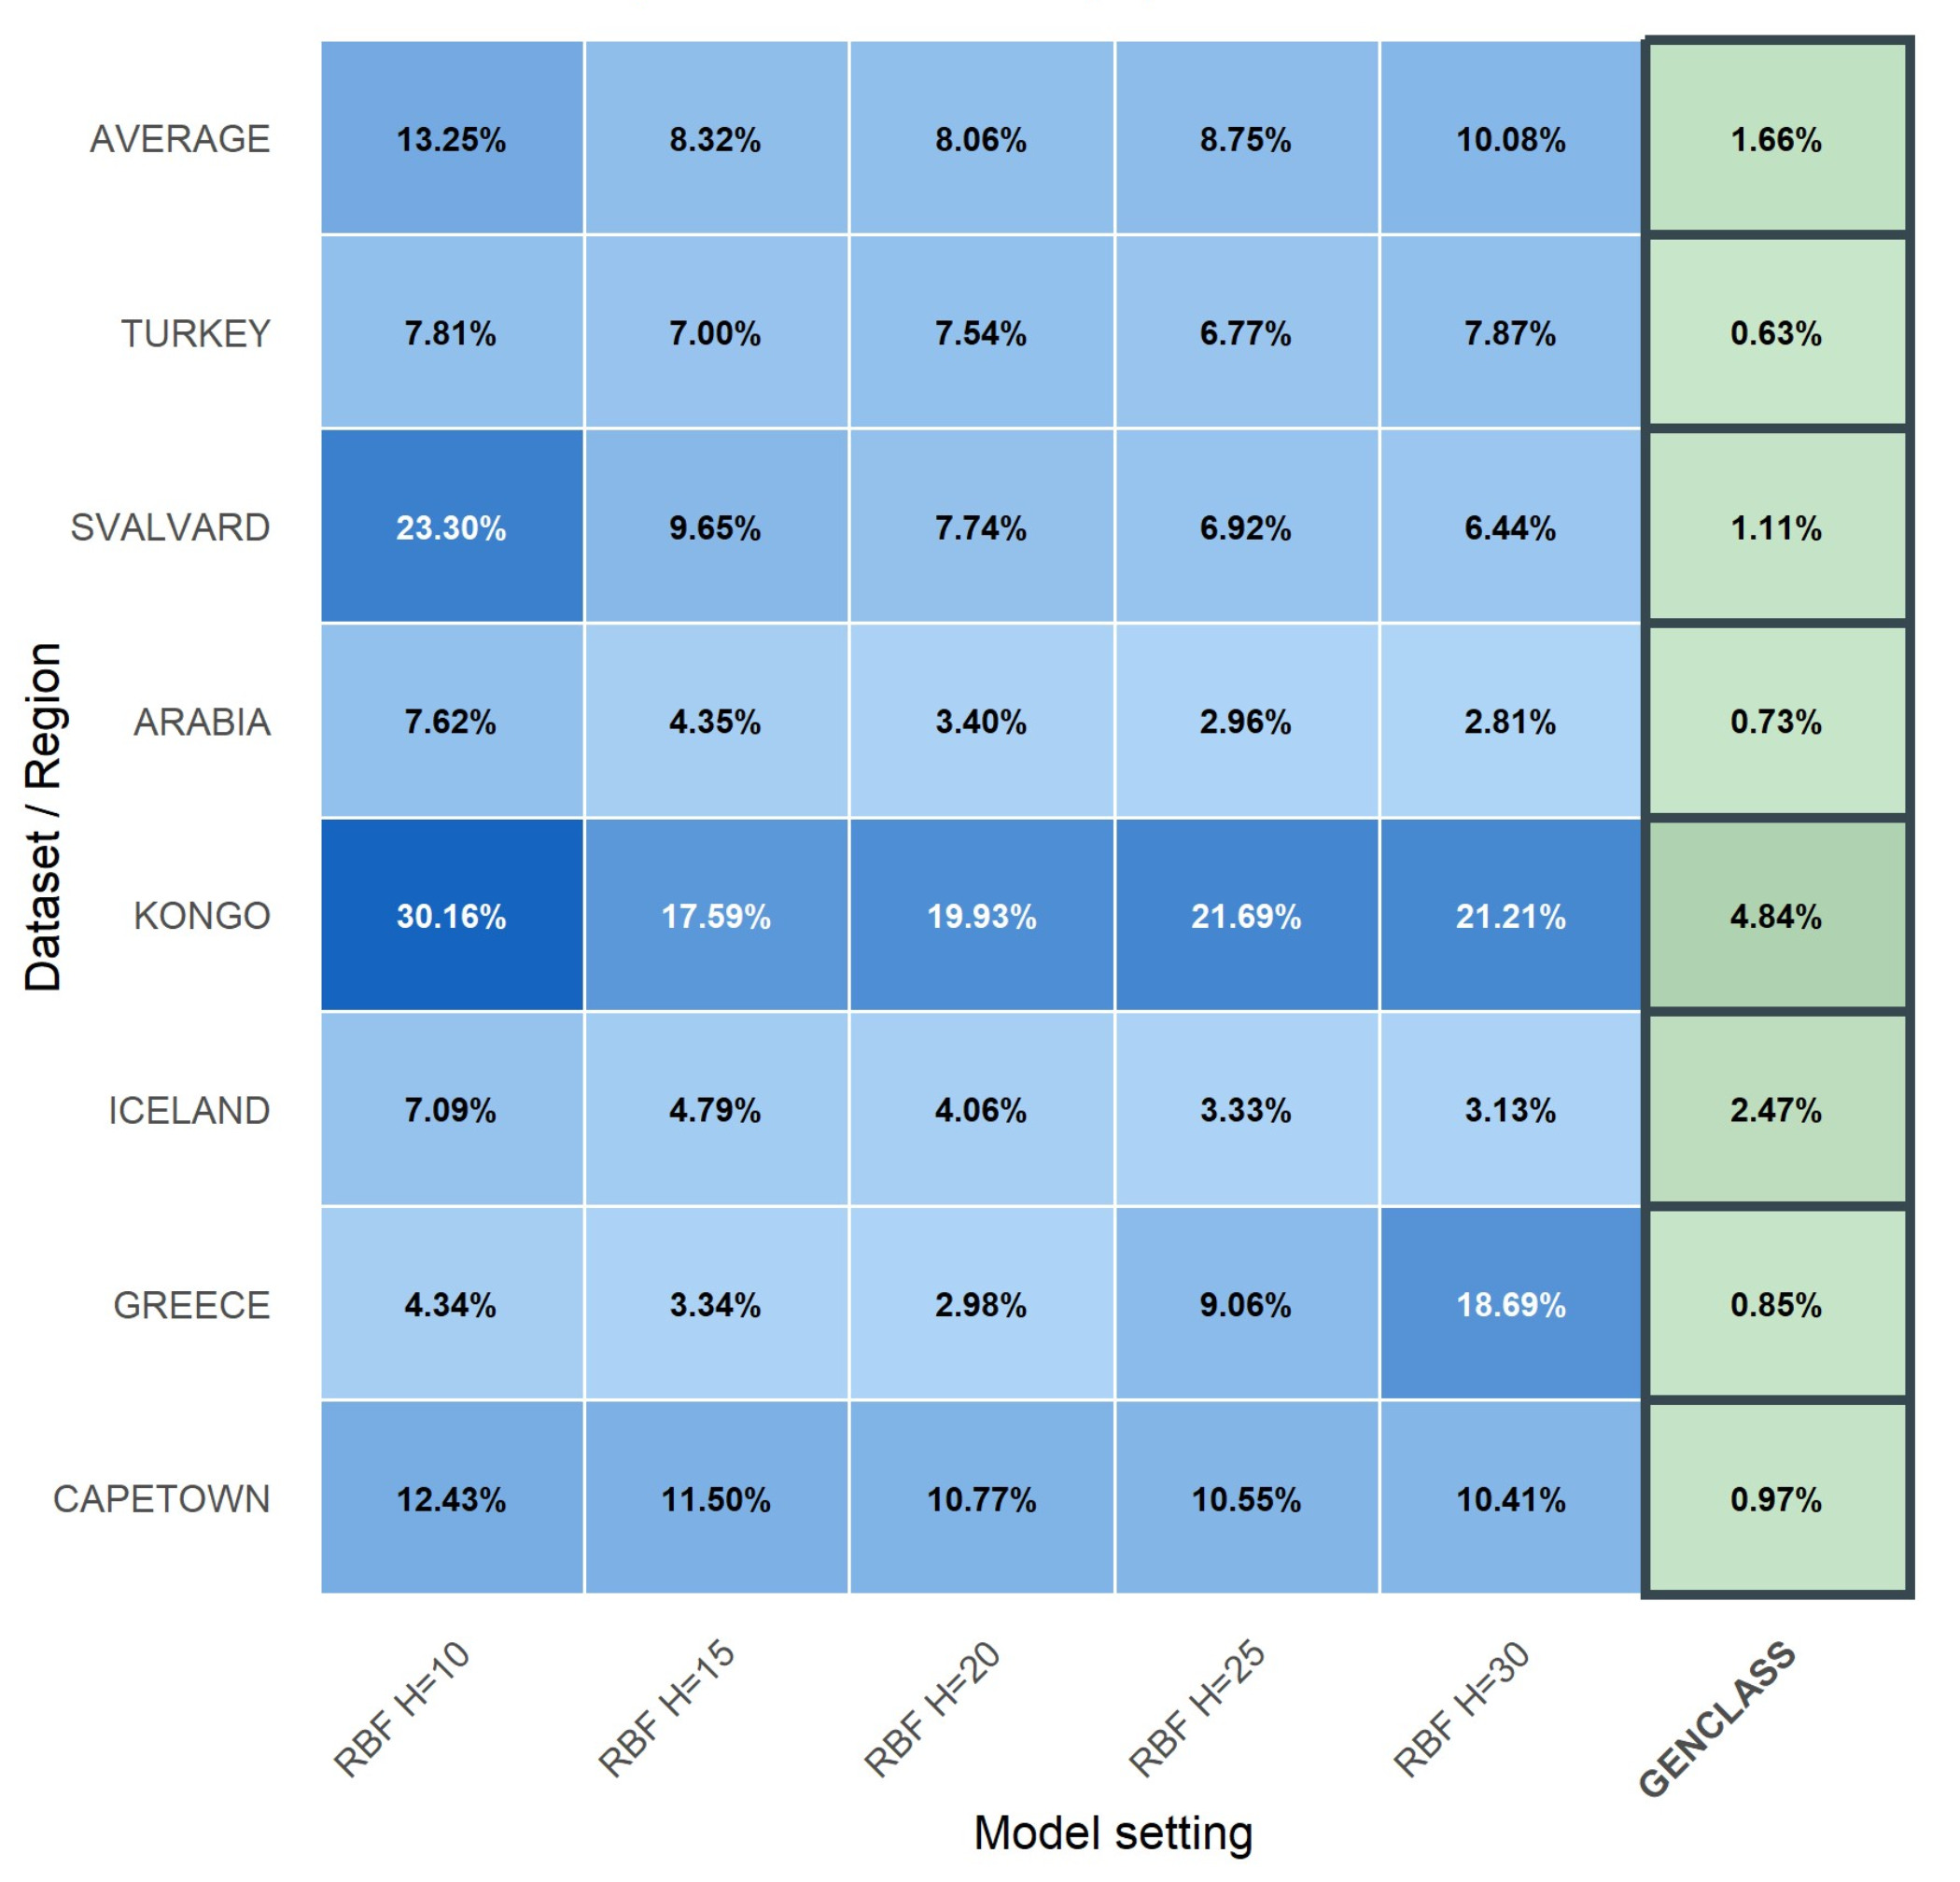
\includegraphics[scale=0.8]{heatMap_RBFvsGENCLASS}

\caption{RBF Sensitivity to the number of hidden (H) nodes and GENCLASS reference \label{fig:RBF-Sensitivity-to}}
\end{figure}

\subsection{Temporal validation}
An additional experiment was conducted to evaluate the reliability of the proposed technique. In this experiment, the datasets were chronologically split, with 80\% of the data used for training and the remaining 20\% used for testing. The GENCLASS method was employed once again, and the experimental results are presented in  \Tabref{table10}.
\begin{table}[H]
	\centering
\begin{tabular}{|c|c|c|c|c|c|c|}
\hline
\textbf{Dataset} &
\centering
GENCLASS\tabularnewline
\hline
\hline
\textbf{Cape Town} & 1.55\% \tabularnewline
\hline
\textbf{Greece} & 0.80\% \tabularnewline
\hline
\textbf{Iceland} & 2.74\% \tabularnewline
\hline
\textbf{Congo} & 3.79\% \tabularnewline
\hline
\textbf{Arabia} & 0.53\% \tabularnewline
\hline
\textbf{Svalbard} & 1.02\%\tabularnewline
\hline
\textbf{Turkey} & 0.44\% \tabularnewline
\hline
\textbf{Average} & \textbf{1.55\%} \tabularnewline
\hline
\end{tabular}
\vspace{1em}
\caption{Presentation of the experimental results for all datasets using the GENCLASS method. In these experiments, the datasets were split chronologically into 80\% training data and 20\% test data.\label{tab:table10}}
\end{table}
The results of this chronological split experiment show that GENCLASS maintains strong performance when temporal ordering is preserved. The average classification error is 1.55\%, which is highly consistent with the 1.66\% average error obtained under the ten-fold cross-validation setting. This indicates that the proposed model does not rely on random temporal mixing and remains reliable when trained on earlier observations and tested on later observations.
\\
Only GENCLASS was evaluated in this additional temporal experiment because the purpose of this section is not to repeat the full comparative benchmark, but to assess the temporal robustness of the proposed method. The full comparison against the baseline models has already been reported in the main experimental evaluation, where GENCLASS achieved the best overall performance. Therefore, the chronological split is included as a targeted validation of the final proposed model under a time-ordered setting.


\clearpage
\section{Conclusions\label{sec:Conclusions}}
The present study provides empirical evidence that daily temperature
time series (1995-2025) across seven regions spanning distinct climate
zones exhibit a consistent warming signal, albeit with pronounced
spatial heterogeneity. Mean temperature increases are not uniform:
Turkey shows the strongest rise, followed by Reykjavik and Greece,
whereas the Congo region displays only marginal changes. This spatial
contrast underscores that large-scale warming manifests differently
depending on geography, seasonality, maritime influence, topography,
and local atmospheric processes (e.g., humidity and cloud-related
dynamics). In methodological terms, the adoption of a region-specific
baseline derived from the early 1995-2000 period proved effective
for defining comparable classes across heterogeneous climates, supporting
relatively balanced class distributions and reducing the risk that
the labeling scheme inherits the already intensified warming of recent
years.

From a modeling perspective, Grammatical Evolution with rule-based
construction (GENCLASS) demonstrates robust and systematic superiority
over the considered baselines (MLP, RBF, SVM, and NNC) across all
datasets, achieving the lowest average classification error and indicating
strong cross-regional generalization. Importantly, the advantage is
not limited to the mean performance but extends to consistency across
markedly different environmental regimes, which is critical for transferability
in climate-related applications. Statistical validation further corroborates
that the observed differences are unlikely to be due to chance: the
overall Friedman test is highly significant (p = 2.49\texttimes 10\textsuperscript{-}\textsuperscript{5}).
Pairwise comparisons indicate that GENCLASS significantly outperforms
SVM and differs significantly from MLP, while differences relative
to RBF and NNC are not statistically significant at the 0.05 level.
This pattern is consistent with GENCLASS remaining competitive against
strong conventional learners while avoiding the pronounced degradation
that some methods exhibit on nonlinear and non-stationary climate
time series.

Sensitivity analyses with respect to key evolutionary parameters strengthen
the methodological credibility of the proposed approach. Increasing
the number of chromosomes$(N_{c})($ and generations ($N_{g}$) yields
systematic error reductions, with clear diminishing returns beyond
approximately$N_{c}$\ensuremath{\approx}500 and $N_{g}$\ensuremath{\approx}1000,
suggesting that improvements stem from enhanced search efficacy rather
than incidental fluctuations. Moreover, the persistent relative difficulty
of the CONGO dataset across all settings is informative: in regions
with weaker temperature seasonality and stronger coupling between
temperature and moisture/cloud processes, a binary temperature-deviation
labeling scheme may be intrinsically harder to learn, motivating either
feature enrichment or a revised labeling strategy that better reflects
the underlying physical dynamics.

The parameter sensitivity analysis indicates that increasing the number
of chromosomes$(N_{c})$ and the number of generations$(N_{g})$ leads
to systematic reductions in error, while the marginal gains progressively
shrink beyond a moderate range of values, revealing clear diminishing
returns. This pattern is expected in genetic and evolutionary computation:
enlarging the computational budget (via larger populations and/or
longer runs) typically improves exploration and convergence at first,
but eventually enters a saturation regime once the search operates
in a sufficiently good region of the solution space. Similar observations
and interpretations have been reported in the literature on parameter
setting/control in evolutionary algorithms, as well as in broader
empirical studies of hyper-parameter spaces that identify wide viable
regions and limited additional benefits beyond certain cost levels
\textit{\cite{Eiben 1999,De Jong 2007,Sipper 2018,O=002019Neill 2018}}.
This contextualization supports reproducibility by documenting that
the selected configuration lies within a stable-performance regime
without requiring excessive computational overhead \textit{\cite{Mills 2014}.}

The effect of the number of generations reported in subsection \ref{subsec:Experiments-with-the}
, Table \ref{tab:Table-8-Experimental-results-on-Ng} and  Figure \ref{fig:The-impact-of-stat-tb18}.
Error decreases strongly as $N_{g}$ increases up to 1000, while the
step from$N_{g}$ =1000 to$N_{g}$ =2000 exhibits a clear flattening
(diminishing returns): the AVERAGE error drops from 1.66\% $\left(N_{g}=1000\right)$
to 1.45\% $\left(N_{g}=2000\right)$, i.e., only by 0.21 percentage
points. For reproducibility and a balanced trade-off between performance
and computational effort, $N_{g}$=1000 is recommended as a practical
default, which is also the value adopted in the main experimental
settings (Table \ref{tabTable-5-:Experimental-settings}). This recommendation
is consistent with the algorithm definition in subsection \ref{subsec:The-proposed-method},
where the maximum number of generations  works as the termination
condition, therefore, computational effort increases approximately
proportionally with the number of generations (for fixed $N_{c}$).
Optionally, an early-stopping rule (e.g., stopping when the best fitness
does not improve for $W$ consecutive generations) can be used to
further balance cost and benefit, while retaining $N_{g}$=1000 as
the default configuration.

Despite the strong results, several limitations delineate the scope
of generalization. First, the data originate from an aggregated provider
and may embed temporal inconsistencies, missing patterns, or changes
in upstream data synthesis over time. Second, evaluation is conducted
using classification error under a binary formulation (Class 0/1),
which necessarily simplifies a multi-factor climate system and does
not quantify predictive uncertainty. Third, careful time-series-aware
evaluation is essential to preclude information leakage from later
periods into earlier ones. Fourth, applying a uniform absolute threshold for class definition while practical may
not be climatically equivalent across tropical versus polar regimes,
where variability and seasonal structure differ qualitatively.

Future work can extend this research along four complementary directions.
First, geographic and climatic coverage should be broadened by incorporating
additional regions per climate zone, explicitly addressing microclimates
(island and mountainous settings), and systematically revisiting Antarctica
through alternative data sources and missing-data strategies. Second,
the representation of the climate system should be enriched by integrating
additional predictors (humidity, pressure, wind, radiation, drought
indices, and teleconnection-related indicators), enabling the learned
rules to capture drivers rather than only temperature outcomes. Third,
the task formulation should be expanded beyond binary classification
toward multi-class regimes and/or regression-based forecasting with
explicit horizons (10/20/30 years) and uncertainty quantification,
thereby improving the operational relevance of the results. Fourth,
experimental protocols should be strengthened with time-aware cross-validation,
decade-wise stability checks, and broader benchmarking against modern
hybrid/deep time-series models, while retaining the interpretability
advantages of rule-based structures. Ultimately, the most impactful
direction is a unified framework that couples predictive accuracy
with statistical rigor and interpretable rules, ensuring that the
resulting climate inferences are not only accurate but also scientifically
explainable and actionable for adaptation planning.
\\
Although the chronological 80/20 hold-out experiment provides a time-ordered validation of the proposed method, future work may further strengthen the evaluation through rolling-window validation, decade-wise stability checks, and broader chronological benchmarking against additional time-series models.



\section*{Acknowledgments}

Not applicable.

\section*{Author Contributions}

Author Contributions:  C.K., V.C. and I.G.T. conceived of the idea and the methodology, and C.K. and V.C. implemented the corresponding software. C.K. conducted the experiments, employing objective functions as test cases, and provided the comparative experiments. V.C. performed the necessary statistical tests. All authors have read and agreed to the published version of the manuscript.


\section*{Funding Statement}

Not applicable.


\section*{Conflict of Interest}
The author(s) declare no conflict of interest.

\section*{Competing Interest}

Not applicable.

\section*{Institutional Review Board Statement}

Not applicable.


\section*{Data Availability}

Available data are included within the manuscript or its supporting materials.


\begin{thebibliography}{10}
\bibitem{Aeschylus}
Aeschylus, 472 B.C.The Persians. Place and date
of edition used as base for this ebook: London: George Allen \& Unwin,
1939. Available from: \url{https://gutenberg.ca/ebooks/murrayaeschylus-persians/murrayaeschylus-persians-00-h.html}

\bibitem{Aeschylus-1}
Aeschylus, 472 B.C. Persians. Richer Resources
Publications, Arlington, Virginia, USA, ISBN 978-1-935238-57-7. Available
from: \url{https://johnstoniatexts.x10host.com/aeschylus/persianshtml.html}

\bibitem{Dey 2021}
 Dey, R., \& Lewis, S. C. Natural disasters linked
to climate change. In: The impacts of climate change. Elsevier, 2021.
p. 177-193. Available from: \url{https://doi.org/10.1016/B978-0-12-822373-4.00004-5.}

\bibitem{Kopitsa}
 Kopitsa, C., Tsoulos, I. G., Miltiadous, A., \&
Charilogis, V. Predicting the Forest Fire Duration Enriched with Meteorological
Data Using Feature Construction Techniques. Symmetry, 2025, 17(11),
1785. \url{https://doi.org/10.3390/sym17111785}

\bibitem{United Nations  2022}
United Nations Environment Programme.
Number of Wildfires to Rise by 50 per Cent by 2100 and Governments
Are Not Prepared, Experts Warn. 23 February 2022. {[}accessed on 7
Novemer 2025{]}. Available from: \url{https://www.unep.org/news-and-stories/press-release/number-wildfires-rise-50-cent-2100-and-governments-are-not-prepared}

\bibitem{United Nations}
 United Nations. Climate Action. {[}accessed
on 7 November 2025{]}.Available from: \url{https://www.un.org/en/climatechange/what-is-climate-change}

\bibitem{United Nations 1992}
 United Nations. Climate Change. United
Nations Framework Convention on Climate Change (UNFCCC). Rio de Janeiro,
Brazil 3 - 14 June 1992. {[}accessed on 7 November 2025{]}. Available
from: \url{https://unfccc.int/process-and-meetings/united-nations-framework-convention-on-climate-change}

\bibitem{United Nations 1997}
 United Nations. Climate Change.The
Kyoto Protocol, 11 December 1997. {[}accessed on 7 November 2025{]}.
Available from: \url{https://unfccc.int/process-and-meetings/the-kyoto-protocol }

\bibitem{United Nations 2015}
United Nations. Climate Action. The
Paris Agreement. {[}accessed on 8 November 2025{]} .Available from:
\url{https://www.un.org/en/climatechange/paris-agreement}

\bibitem{NASA 2024}
 NASA. Global Temperature - Earth Indicator. 2024.
{[}accessed on 8 November 2025{]}. Available from: \url{https://science.nasa.gov/earth/explore/earth-indicators/global-temperature/}

\bibitem{Arrhenius}
 Arrhenius, S. On the Influence of Carbonic Acid
in the Air upon the Temperature of the Ground. Philosophical Magazine
and Journal of Science, 1896. Series 5, Volume 41, April 1896, pages
237-276. A

\bibitem{Rolnick 2022} 
Rolnick, D., Donti, P. L., Kaack, L. H., Kochanski,
K., Lacoste, A., Sankaran, K., ... \& Bengio, Y. Tackling climate
change with machine learning. ACM Computing Surveys (CSUR), 2022.
55(2), 1-96.

\bibitem{Koulelis 2023}
 Koulelis, P. P., Proutsos, N., Solomou, A.
D., Avramidou, E. V., Malliarou, E., Athanasiou, M., ... \& Petrakis,
P. V. Effects of climate change on Greek forests: A review. Atmosphere,
2023. 14(7), 1155.

\bibitem{Rovithakis 2022}
 Rovithakis, A., Grillakis, M. G., Seiradakis,
K. D., Giannakopoulos, C., Karali, A., Field, R., ... \& Voulgarakis,
A. Future climate change impact on wildfire danger over the Mediterranean:
the case of Greece. Environmental Research Letters, 2022. 17(4), 045022.

\bibitem{Xepapadeas 2024}
 Xepapadeas, P., Douvis, K., Kapsomenakis,
I., Xepapadeas, A., \& Zerefos, C. Wildfires, Vulnerability, and Climate
Change: Methodology and Application to the Regions of Greece. 2024.
Available from: \url{doi: 10.20944/preprints202405.0081.v1}

\bibitem{Knox 2000}
 Knox, J. C. Sensitivity of modern and Holocene
floods to climate change. Quaternary Science Reviews, 2000. 19(1-5),
439-457.

\bibitem{Milly 2002}
 Milly, P. C. D., Wetherald, R. T., Dunne, K.
A., \& Delworth, T. L. Increasing risk of great floods in a changing
climate. Nature, 2002. 415(6871), 514-517.

\bibitem{Angra 2022} 
Angra, D., \& Sapountzaki, K. Climate change
affecting forest fire and flood risk---facts, predictions, and perceptions
in Central and South Greece. Sustainability, 2022, 14.20: 13395. Available
from: \url{https://doi.org/10.3390/su142013395}

\bibitem{Cook 2018}
 Cook, B. I., Mankin, J. S., \& Anchukaitis, K.
J. Climate change and drought: From past to future. Current Climate
Change Reports,2018. 4(2), 164-179.

\bibitem{Stathi 2023}
 Stathi, E., Kastridis, A., \& Myronidis, D.Analysis
of hydro meteorological trends and drought severity in water-demanding
Mediterranean islands under climate change conditions. Climate, 2023,
11.5: 106. Available from: \url{https://doi.org/10.3390/cli11050106}

\bibitem{Yuan 2023} 
Yuan, X., Wang, Y., Ji, P., Wu, P., Sheffield, J.,
\& Otkin, J. A. A global transition to flash droughts under climate
change. Science, 2023. 380(6641), 187-191.

\bibitem{Kretschmer 2017}
 Kretschmer, M., Runge, J., \& Coumou, D.
Early prediction of extreme stratospheric polar vortex states based
on causal precursors. Geophysical research letters, 2017. 44(16),
8592-8600. Available from: \url{ https://doi.org/10.1002/2017GL074696}

\bibitem{Kambezidis 2021}
 Kambezidis, H. D., Psiloglou, B. E., Varotsos,
K. V., \& Giannakopoulos, C. Climate change and thermal comfort in
Greece. Climate, 2021, 9.1: 10. Available from: \url{ https://doi.org/10.3390/cli9010010}

\bibitem{Lindsey 2025}
 Lindsey, R. Dahlman, L. Climate change: global
temperature. NOAA. Science \& Information for Climate-Smart nation.
2025. {[}accessed on 19 March 2026{]}. Available from:\url{https://www.climate.gov/news-features/understanding-climate/climate-change-global-temperature}

\bibitem{Mansfield 2020}
 Mansfield, L. A., Nowack, P. J., Kasoar,
M., Everitt, R. G., Collins, W. J., \& Voulgarakis, A. Predicting
global patterns of long-term climate change from short-term simulations
using machine learning. npj Climate and Atmospheric Science, 2020.
3(1), 44.

\bibitem{Haggag 2021} 
Haggag, M., Siam, A. S., El-Dakhakhni, W.,
Coulibaly, P., \& Hassini, E. A deep learning model for predicting
climate-induced disasters. Natural Hazards, 2021. 107(1), 1009-1034.

\bibitem{Haq 2022}
 Haq, M. A. CDLSTM: A novel model for climate change
forecasting. Computers, Materials \& Continua, 2022. 71(2).

\bibitem{Slater 2023}
 Slater, L. J., Arnal, L., Boucher, M. A., Chang,
A. Y. Y., Moulds, S., Murphy, C., ... \& Zappa, M. Hybrid forecasting:
blending climate predictions with AI models. Hydrology and earth system
sciences, 2023. 27(9), 1865-1889.

\bibitem{Bist 2024} 
Bist, A. S., Rawat, B., Joshi, Y., Aini, Q.,
Santoso, N. P. L., \& Kusumawardhani, D. A. R. . Harnessing Deep Learning
for Accurate Climate Change Predictions. In 2024 3rd International
Conference on Creative Communication and Innovative Technology (ICCIT)
(2024, August) (pp. 1-6). IEEE.

\bibitem{GAUTAM 2025}
GAUTAM, A., AJMERA, R., DHARAMDASANI, D. K.,
SRIVASTAVA, S., \& JOHARI, A. IMPROVING CLIMATE CHANGE PREDICTIONS
USING TIME SERIES ANALYSIS AND DEEP LEARNING. Global \& Stochastic
Analysis, 2025. 12(4).

\bibitem{O'Neill 2002}
O'Neill, M., \& Ryan, C. Grammatical evolution.
IEEE Transactions on Evolutionary Computation, 2002. 5(4), 349-358.

\bibitem{Kramer 2017}
Kramer, O. Genetic algorithms. In Genetic algorithm
essentials. Cham: Springer International Publishing. 2017. pp. 11-19.

\bibitem{Backus 1959}
Backus, J. W. The syntax and the semantics of
the proposed international algebraic language of the Zurich ACM-GAMM
Conference. 1959. In ICIP Proceedings (pp. 125-132).

\bibitem{Ryan 1998}
Ryan, C., Collins, J. J., \& Neill, M. O. Grammatical
evolution: Evolving programs for an arbitrary language. In European
conference on genetic programming 1998. (pp. 83-96). Berlin, Heidelberg:
Springer (1998, April) Berlin Heidelberg.

\bibitem{Neill 1999}
O\textquoteright Neill, M., \& Ryan, C.. Evolving
multi-line compilable C programs. In European Conference on Genetic
Programming 1999. (pp. 83-92). Berlin, Heidelberg: Springer (1999,
May) Berlin Heidelberg.

\bibitem{Brabazon 2006}
Brabazon, A., \& O'Neill, M. Credit classification
using grammatical evolution. Informatica, 2006. 30(3).

\bibitem{Sen 2009}
Sen, S., \& Clark, J. A. . A grammatical evolution
approach to intrusion detection on mobile ad hoc networks. In Proceedings
of the second ACM conference on Wireless network security2009. (pp.
95-102). (2009, March).

\bibitem{Chen 2008}
Chen, L., Tan, C. H., Kao, S. J., \& Wang, T.
S. Improvement of remote monitoring on water quality in a subtropical
reservoir by incorporating grammatical evolution with parallel genetic
algorithms into satellite imagery. Water Research, 2008. 42(1-2),
296-306.

\bibitem{Hidalgo 2014}
Hidalgo, J. I., Colmenar, J. M., Risco-Martin,
J. L., Cuesta-Infante, A., Maqueda, E., Botella, M., \& Rubio, J.
A. Modeling glycemia in humans by means of grammatical evolution.
Applied Soft Computing, 2014. 20, 40-53.

\bibitem{Tavares 2012}
Tavares, J., \& Pereira, F. B. . Automatic
design of ant algorithms with grammatical evolution. In European conference
on genetic programming 2012. (pp. 206-217). Berlin, Heidelberg: Springer
(2012, April) Berlin Heidelberg.

\bibitem{Zapater 2016}
Zapater, M., Risco-Martín, J. L., Arroba, P.,
Ayala, J. L., Moya, J. M., \& Hermida, R. Runtime data center temperature
prediction using grammatical evolution techniques. Applied Soft Computing,
2016. 49, 94-107.

\bibitem{Ryan 1998-1}
Ryan, C., O\textquoteright Neill, M., \& Collins,
J. J. Grammatical evolution: Solving trigonometric identities. In
proceedings of Mendel 1998. (Vol. 98, p. 4th). Brno, Czech Republic:
Technical University of Brno, (1998, June) Faculty of Mechanical Engineering.

\bibitem{de la Puente 2002}
de la Puente, A. O., Alfonso, R. S., \&
Moreno, M. A. Automatic composition of music by means of grammatical
evolution. In Proceedings of the 2002 conference on APL: array processing
languages: lore, problems, and applications 2002. (pp. 148-155).

\bibitem{De Campos 2016}
De Campos, L. M. L., de Oliveira, R. C. L.,
\& Roisenberg, M. Optimization of neural networks through grammatical
evolution and a genetic algorithm. Expert Systems with Applications,
2016. 56, 368-384.

\bibitem{Soltanian 2022}
Soltanian, K., Ebnenasir, A., \& Afsharchi,
M. Modular grammatical evolution for the generation of artificial
neural networks. Evolutionary computation, 2022. 30(2), 291-327

\bibitem{Dempsey 2007}
Dempsey, I., O'Neill, M., \& Brabazon, A. Constant
creation in grammatical evolution. International Journal of Innovative
Computing and Applications, 2007. 1(1), 23-38.

\bibitem{Galv=0000E1n-L=0000F3pez 2010}
Galvan-Lopez, E., Swafford,
J. M., O\textquoteright Neill, M., \& Brabazon, A. Evolving a ms.
pacman controller using grammatical evolution. In European Conference
on the Applications of Evolutionary Computation 2010 (pp. 161-170).
Berlin, Heidelberg: Springer (2010, April). Berlin Heidelberg.

\bibitem{Shaker 2012}
Shaker, N., Nicolau, M., Yannakakis, G. N.,
Togelius, J., \& O'neill, M. Evolving levels for super mario bros
using grammatical evolution. In 2012 IEEE Conference on Computational
Intelligence and Games (CIG) (pp. 304-311).(2012, September). IEEE.

\bibitem{Mart=0000EDnez=002010Rodr=0000EDguez 2020}
Martínez-Rodriguez,
D., Colmenar, J. M., Hidalgo, J. I., Villanueva Mico, R. J., and Salcedo-Sanz,
S. Particle swarm grammatical evolution for energy demand estimation.
Energy Science and Engineering, 2020. 8(4), 1068-1079.

\bibitem{Sabar 2013}
Sabar, N. R., Ayob, M., Kendall, G., \& Qu, R.
Grammatical evolution hyper-heuristic for combinatorial optimization
problems. IEEE Transactions on Evolutionary Computation, 2013. 17(6),
840-861.

\bibitem{Ryan 2022}
Ryan, C., Kshirsagar, M., Vaidya, G., Cunningham,
A., \& Sivaraman, R. Design of a cryptographically secure pseudo random
number generator with grammatical evolution. Scientific reports, 2022.
12(1), 8602.

\bibitem{Pereira 2021}
Pereira, P. J., Cortez, P., \& Mendes, R. Multi-objective
grammatical evolution of decision trees for mobile marketing user
conversion prediction. Expert Systems with Applications,2021. 168,
114287.

\bibitem{Castej=0000F3n 2018}
Castejon, F., \& Carmona, E. J. Automatic
design of analog electronic circuits using grammatical evolution.
Applied Soft Computing, 2018. 62, 1003-1018.


\bibitem{EM-DATA}
EM-DATA. The International Disaster Database. Emergency
Events Database. {[}accessed on 9 November 2025{]}. Available from:
\url{https://www.emdat.be/}

\bibitem{Visual Crossing}
 Historical Weather Data. {[accessed on 13 December{]}. 
	Available from \url{https://www.visualcrossing.com/}

\bibitem{Tsoulos 2020}
 Tsoulos, I.G. Creating classification rules
using grammatical evolution. Int. J. Comput. Intell. Stud. 2020, 9,
161--171.

\bibitem{Anastasopoulos 2021}
Anastasopoulos, N.; Tsoulos, I.G.; Tzallas,
A. GenClass: A parallel tool for data classification based on Grammatical
Evolution. SoftwareX 2021, 16, 100830.

\bibitem{GitHub}
GEN CLASS. {[accessed on 18 April 2026{]}.
	Available from \url{https://github.com/itsoulos/GenClass/}

\bibitem{Poli 1998}
Poli, R., \& Langdon, W. B. Genetic programming
with one-point crossover 1998. (pp. 180-189). Springer London

\bibitem{Tsoulos 2025}
Tsoulos, I. G., Charilogis, V., Kyrou, G.,
Stavrou, V. N., \& Tzallas, A. OPTIMUS: A Multidimensional Global
Optimization Package. Journal of Open Source Software, 2025. 10(108),
7584. Available from \url{https://github.com/itsoulos/GlobalOptimus/}

\bibitem{M.J.D Powell 1989}
M.J.D Powell, A Tolerant Algorithm for
Linearly Constrained Optimization Calculations, Mathematical Programming
\textbf{45}, pp. 547-566, 1989.

\bibitem{J. Park 1991}
J. Park and I. W. Sandberg, Universal Approximation
Using Radial-Basis-Function Networks, Neural Computation \textbf{3},
pp. 246-257, 1991.

\bibitem{G.A. Montazer 2018}
G.A. Montazer, D. Giveki, M. Karami,
H. Rastegar, Radial basis function neural networks: A review. Comput.
Rev. J \textbf{1}, pp. 52-74, 2018.

\bibitem{Chang 2011}
Chang, C. C., \& Lin, C. J. LIBSVM: A library
for support vector machines. ACM transactions on intelligent systems
and technology, 2011. (TIST), 2(3), 1-27.

\bibitem{Tsoulos 2008}
Tsoulos, I., Gavrilis, D., \& Glavas, E. Neural
network construction and training using grammatical evolution. Neurocomputing,
2008. 72(1-3), 269-277.

\bibitem{xgboost}Tianqi Chen and Carlos Guestrin. XGBoost: A Scalable Tree Boosting System. In 22nd SIGKDD Conference on Knowledge Discovery and Data Mining, 2016

\bibitem{bayesnn}Cantin, R. BayesOpt: A Bayesian Optimization Library for Nonlinear Optimization, Experimental Design and Bandits. J. Mach. Learn. Res. 2014, 15,3735-3739.



\bibitem{adagrad}Ward, R.; Wu, X.; Bottou, L. Adagrad stepsizes: Sharp convergence over nonconvex landscapes. J. Mach. Learn. Res. 2020, 21, 1-30.

\bibitem{Eiben 1999}
Eiben, A. E., Hinterding, R., \&amp; Michalewicz,
Z. Parameter control in evolutionary algorithms. IEEE Transactions
on Evolutionary Computation, 1999. 3(2), 124--141.

\bibitem{De Jong 2007}
De Jong, K. A. Parameter setting in EAs: A
30 year perspective. In F. G. Lobo, C. F. Lima, \&amp; Z. Michalewicz
(Eds.), Parameter Setting in Evolutionary Algorithms2007. (pp. 1--18).
Springer.

\bibitem{Sipper 2018}
Sipper, M., Fu, W., Ahuja, K., \&amp; Moore,
J. H. Investigating the parameter space of evolutionary algorithms.
BioData Mining, 2018. 11, 2.

\bibitem{O=002019Neill 2018}
O\textquoteright Neill, M., Brabazon,
A., Nicolau, M., McGarraghy, S., \&amp; Keenan, P. (Eds.). The Handbook
of Grammatical Evolution. 2018. Springer.

\bibitem{Mills 2014}
Mills, K. L., Filliben, J. J., \&amp; Haines,
A. Determining relative importance and best settings for genetic algorithm
control parameters. Evolutionary Computation, 2014. 23(2), 309--342.

}}\end{thebibliography}



\end{document}
